%%-----------------------------------------------------------------------------
%%
%%                                   Sean Mauch
%%                       California Institute of Technology
%%                       (a) 2000-2004 No Rights Reserved
%%
%%-----------------------------------------------------------------------------

\flushbottom


%% CONTINUE: update notation for interval from (,) to ( .. ).


%%============================================================================
%%============================================================================
\chapter{Differential Calculus}
\label{chapter_differential}
\index{differential calculus}



%%============================================================================
\section{Limits of Functions}
\index{limits of functions}


%% CONT motivate

\paragraph{Definition of a Limit.}
If the value of the function $y(x)$ gets arbitrarily close to $\psi$ as 
$x$ approaches the point $\xi$, then we say that the limit of the function
as $x$ approaches $\xi$ is equal to $\psi$.  This is written:
\[
\lim_{x \to \xi} y(x) = \psi
\]
Now we make the notion of ``arbitrarily close'' precise.  For any $\epsilon > 0$
there exists a $\delta > 0$ such that $|y(x) - \psi| < \epsilon$ for all
$0 < | x - \xi | < \delta$.  That is, there is an interval surrounding the
point $x = \xi$ for which the function is within $\epsilon$ of $\psi$.
See Figure~\ref{limfx}.  Note that the interval surrounding $x = \xi$ is
a deleted neighborhood, that is it does not contain the point $x = \xi$.
Thus the value of the function at $x = \xi$ need not be equal to $\psi$ for 
the limit to exist.  Indeed the function need not even be defined 
at $x = \xi$.


\begin{figure}[h!]
  \begin{center}
    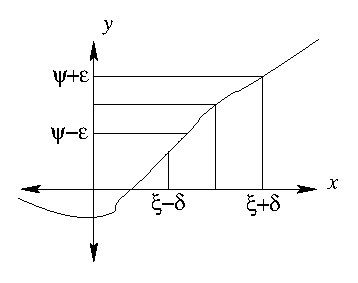
\includegraphics[width=0.33\textwidth]{calculus/differential/limfx}
  \end{center}
  \caption{The neighborhood of the point.}
  \label{limfx}
\end{figure}



To prove that a function has a limit at a point $\xi$ we first bound 
$|y(x) - \psi|$ in terms of $\delta$ for values of $x$ satisfying
$0 < |x - \xi| < \delta$.  Denote this upper bound by $u(\delta)$.  
Then for an arbitrary $\epsilon > 0$, we determine a $\delta > 0$ such that 
the the upper bound $u(\delta)$ and hence $|y(x) - \psi|$ is less than
$\epsilon$.




\begin{Example}
  Show that 
  \[
  \lim_{x \to 1} x^2 = 1.
  \]
  Consider any $\epsilon > 0$.  We need to show that there exists a $\delta > 0$
  such that $|x^2 - 1| < \epsilon$ for all $|x-1| < \delta$.  First we obtain
  a bound on $|x^2 - 1|$.
  \begin{align*}
    |x^2 - 1|
    &= | (x-1)(x+1) | \\
    &= | x-1 | | x+1 | \\
    &< \delta | x+1 | \\
    &= \delta |(x-1) + 2| \\
    &< \delta ( \delta + 2 ) 
  \end{align*}
  Now we choose a positive $\delta$ such that,
  \[
  \delta ( \delta + 2 ) = \epsilon.
  \]
  We see that
  \[
  \delta = \sqrt{1 + \epsilon} - 1,
  \]
  is positive and satisfies the criterion that $|x^2 - 1| < \epsilon$ for all
  $0 < |x-1| < \delta$.  Thus the limit exists.
\end{Example}






\begin{Example}
  \label{yxineqlim}
  Recall that the value of the function $y(\xi)$ need not be equal to 
  $\lim_{x \to \xi} y(x)$ for the limit to exist.  We show an example of this.
  Consider the function
  \[
  y(x) = 
  \begin{cases}
    1 & \mathrm{for}\ x \in \setZ, \\
    0 & \mathrm{for}\ x \not\in \setZ.
  \end{cases}
  \]
  For what values of $\xi$ does $\lim_{x \to \xi} y(x)$ exist?

  First consider $\xi \not\in \setZ$.  Then there exists an open 
  neighborhood $a<\xi<b$ around $\xi$ such that $y(x)$ is identically zero for
  $x \in (a,b)$.  Then trivially, $\lim_{x \to \xi} y(x) = 0$.

  Now consider $\xi \in \setZ$.  Consider any $\epsilon > 0$.  Then if
  $|x - \xi| < 1$ then $|y(x) - 0| = 0 < \epsilon$.  Thus we see that
  $\lim_{x \to \xi} y(x) = 0$.

  Thus, regardless of the value of $\xi$, $\lim_{x \to \xi} y(x) = 0$.
\end{Example}




\paragraph{Left and Right Limits.}
\index{limit!left and right}
With the notation $\lim_{x \to \xi^+} y(x)$ we denote the right limit of 
$y(x)$.  This is the limit as $x$ approaches $\xi$ from above.  
Mathematically: $\lim_{x \to \xi^+}$ exists if for any $\epsilon > 0$ 
there exists a $\delta > 0$ such that $|y(x) - \psi| < \epsilon$ for all 
$0 < \xi - x < \delta$.  The left limit $\lim_{x \to \xi^-} y(x)$ is 
defined analogously.



\begin{Example}
  Consider the function, $\frac{\sin x}{|x|}$, defined for $x \neq 0$.  
  (See Figure~\ref{sinxabsx}.)
  The left and right limits exist as $x$ approaches zero.
  \[
  \lim_{x \to 0^+} \frac{\sin x}{|x|} = 1, \qquad
  \lim_{x \to 0^-} \frac{\sin x}{|x|} = -1 
  \]
  However the limit, 
  \[
  \lim_{x \to 0} \frac{\sin x}{|x|},
  \]
  does not exist.
  \begin{figure}[h!]
    \begin{center}
      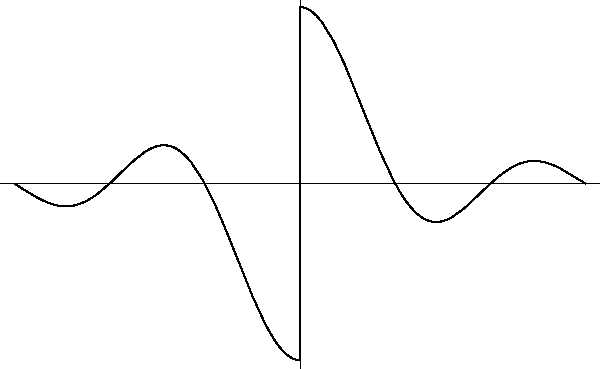
\includegraphics[width=0.33\textwidth]{calculus/differential/sinxabsx}
    \end{center}
    \caption{The function has left and right limits at the origin.}
    \label{sinxabsx}
  \end{figure}
\end{Example}







\paragraph{Properties of Limits.}
Let $\displaystyle \lim_{x \to \xi} f(x)$ and $\displaystyle \lim_{x \to \xi} g(x)$ 
exist.
\begin{itemize}
\item
  $\displaystyle 
  \lim_{x \to \xi} \left( a f(x) + b g(x) \right)
  = a \lim_{x \to \xi} f(x) + b \lim_{x \to \xi} g(x)
  $.
\item
  $\displaystyle 
  \lim_{x \to \xi} \left( f(x) g(x) \right)
  = \left(\lim_{x \to \xi} f(x) \right) \left( \lim_{x \to \xi} g(x) \right)
  $.
\item
  $\displaystyle 
  \lim_{x \to \xi} \left( \frac{f(x)}{g(x)} \right)
  = \frac{\lim_{x \to \xi} f(x)}{\lim_{x \to \xi} g(x)}
  $ 
  if 
  $\displaystyle 
  \lim_{x \to \xi} g(x) \neq 0
  $.
\end{itemize}





\begin{Example}
  We prove that if $\lim_{x \to \xi} f(x) = \phi$ and $\lim_{x \to \xi} g(x) = \gamma$ 
  exist then
  \[
  \lim_{x \to \xi} \left( f(x) g(x) \right)
  = \left(\lim_{x \to \xi} f(x) \right) \left( \lim_{x \to \xi} g(x) \right).
  \]
  Since the limit exists for $f(x)$, we know that for all $\epsilon > 0$ there 
  exists $\delta > 0$ such that $|f(x) - \phi| < \epsilon$ for $|x - \xi| < \delta$.  Likewise
  for $g(x)$.
  We seek to show that for all $\epsilon > 0$ there exists $\delta > 0$ such that
  $|f(x) g(x) - \phi \gamma| < \epsilon$ for $|x - \xi| < \delta$.  We proceed by writing
  $|f(x) g(x) - \phi \gamma|$, in terms of $|f(x) - \phi|$ and $|g(x) - \gamma|$, which
  we know how to bound.
  \begin{align*}
    | f(x) g(x) - \phi \gamma | 
    &= | f(x) (g(x) - \gamma) + (f(x) - \phi) \gamma | \\
    &\leq | f(x) | | g(x) - \gamma | + | f(x) - \phi | | \gamma |
  \end{align*}
  If we choose a $\delta$ such that $| f(x) | | g(x) - \gamma | < \epsilon / 2$ and 
  $| f(x) - \phi | | \gamma | < \epsilon / 2$ then we will have the desired 
  result: $| f(x) g(x) - \phi \gamma | < \epsilon$.
  Trying to ensure that $| f(x) | | g(x) - \gamma | < \epsilon / 2$ is hard because
  of the $|f(x)|$ factor.  We will replace that factor with a constant.
  We want to write $| f(x) - \phi | | \gamma | < \epsilon / 2$ as $| f(x) - \phi | < \epsilon / (2 |\gamma|)$,
  but this is problematic for the case $\gamma = 0$.  We fix these two problems
  and then proceed.  We choose $\delta_1$ such that $|f(x) - \phi| < 1$ for 
  $|x - \xi| < \delta_1$.  This gives us the desired form.
  \[
  | f(x) g(x) - \phi \gamma | 
  \leq (|\phi| + 1) | g(x) - \gamma | + | f(x) - \phi | (| \gamma | + 1),\ 
  \mathrm{for}\ |x - \xi| < \delta_1
  \]
  Next we choose $\delta_2$ such that $|g(x) - \gamma| < \epsilon / (2 (|\phi| + 1))$ for
  $|x - \xi| < \delta_2$ and choose $\delta_3$ such that $|f(x) - \phi| < \epsilon / (2 (|\gamma| + 1))$ 
  for $|x - \xi| < \delta_3$.
  Let $\delta$ be the minimum of $\delta_1$, $\delta_2$ and $\delta_3$.
  \begin{gather*}
    | f(x) g(x) - \phi \gamma | 
    \leq (|\phi| + 1) | g(x) - \gamma | + | f(x) - \phi | (| \gamma | + 1)
    < \frac{\epsilon}{2} + \frac{\epsilon}{2},\ 
    \mathrm{for}\ |x - \xi| < \delta
    \\
    | f(x) g(x) - \phi \gamma | < \epsilon,\ \mathrm{for}\ |x - \xi| < \delta
  \end{gather*}
  We conclude that the limit of a product is the product of the limits.
  \[
  \lim_{x \to \xi} \left( f(x) g(x) \right)
  = \left(\lim_{x \to \xi} f(x) \right) \left( \lim_{x \to \xi} g(x) \right)
  = \phi \gamma.
  \]
\end{Example}



\begin{Result}
  \textbf{Definition of a Limit.}
  The statement: 
  \[
  \lim_{x \to \xi} y(x) = \psi
  \]
  means that $y(x)$ gets arbitrarily close to $\psi$ as $x$ approaches $\xi$.
  For any $\epsilon > 0$ there exists a $\delta > 0$ such that 
  $|y(x) - \psi| < \epsilon$ for all $x$ in the neighborhood 
  $0 < | x - \xi | < \delta$.  The left and right limits,
  \[
  \lim_{x \to \xi^-} y(x) = \psi \quad \mathrm{and} \quad
  \lim_{x \to \xi^+} y(x) = \psi
  \]
  denote the limiting value as $x$ approaches $\xi$ respectively from 
  below and above.  The neighborhoods are respectively $-\delta < x - \xi < 0$ 
  and $0 < x - \xi < \delta$.

  \textbf{Properties of Limits.}
  Let $\displaystyle \lim_{x \to \xi} u(x)$ and 
  $\displaystyle \lim_{x \to \xi} v(x)$ exist.
  \begin{itemize}
  \item
    $\displaystyle 
    \lim_{x \to \xi} \left( a u(x) + b v(x) \right)
    = a \lim_{x \to \xi} u(x) + b \lim_{x \to \xi} v(x)
    $.
  \item
    $\displaystyle 
    \lim_{x \to \xi} \left( u(x) v(x) \right)
    = \left(\lim_{x \to \xi} u(x) \right) \left( \lim_{x \to \xi} v(x) \right)
    $.
  \item
    $\displaystyle 
    \lim_{x \to \xi} \left( \frac{u(x)}{v(x)} \right)
    = \frac{\lim_{x \to \xi} u(x)}{\lim_{x \to \xi} v(x)}
    $ 
    if 
    $\displaystyle 
    \lim_{x \to \xi} v(x) \neq 0
    $.
  \end{itemize}
\end{Result}





%%============================================================================
\section{Continuous Functions}
\index{continuous functions}



\paragraph{Definition of Continuity.}
\index{continuity}
A function $y(x)$ is said to be \textit{continuous at} $x = \xi$ if
the value of the function is equal to its limit, that is,
$\lim_{x \to \xi} y(x) = y(\xi)$.  Note that this one condition is 
actually the three conditions: $y(\xi)$ is defined, $\lim_{x \to \xi} y(x)$
exists and $\lim_{x \to \xi} y(x) = y(\xi)$.  A function is \textit{continuous}
if it is continuous at each point in its domain.  A function is 
\textit{continuous on the closed interval} $[a,b]$ if the function is 
continuous for each point $x \in (a,b)$ and $\lim_{x \to a^+} y(x) = y(a)$
and $\lim_{x \to b_-} y(x) = y(b)$.



\paragraph{Discontinuous Functions.}
\index{discontinuous functions}
If a function is not continuous at a point it is called \textit{discontinuous}
at that point.  If $\lim_{x \to \xi} y(x)$ exists but is not equal to 
$y(\xi)$, then the function has a \textit{removable discontinuity}.  It 
is thus named because we could define a continuous function
\[
z(x) = 
\begin{cases}
  y(x) & \mathrm{for}\ x \neq \xi, \\
  \lim_{x \to \xi} y(x) & \mathrm{for}\ x = \xi,
\end{cases}
\]
to remove the discontinuity.  If both the left and right limit of a function
at a point exist, but are not equal, then the function has a 
\textit{jump discontinuity} at that point.  If either the left or right
limit of a function does not exist, then the function is said to have an
\textit{infinite discontinuity} at that point.




\begin{Example}
  $\frac{\sin x}{x}$ has a removable discontinuity at $x=0$.  
  The Heaviside function,
  \[
  H(x) = 
  \begin{cases}
    0 & \mathrm{for}\ x < 0, \\
    1/2 & \mathrm{for}\ x = 0, \\
    1 & \mathrm{for}\ x > 0,
  \end{cases}
  \]
  has a jump discontinuity at $x = 0$.  $\frac{1}{x}$ has an infinite
  discontinuity at $x = 0$.  See Figure~\ref{discont}.
  \begin{figure}[h!]
    \begin{center}
      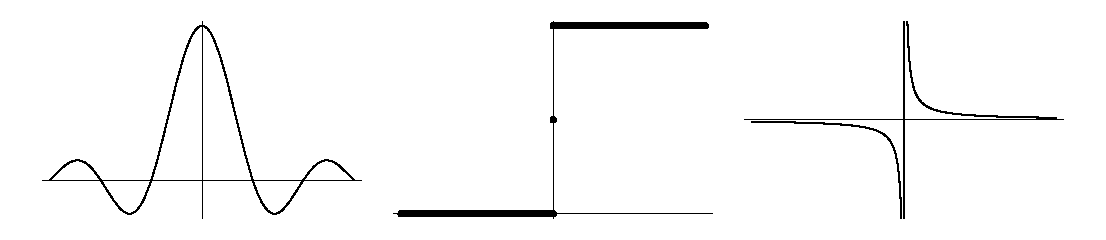
\includegraphics[width=0.9\textwidth]{calculus/differential/discont}
    \end{center}
    \caption{A removable discontinuity, a jump discontinuity and an 
      infinite discontinuity.}
    \label{discont}
  \end{figure}
\end{Example}





\paragraph{Properties of Continuous Functions.}
\begin{description}
  %%
\item{Arithmetic.}
  If $u(x)$ and $v(x)$ are continuous at $x = \xi$ then $u(x) \pm v(x)$ and
  $u(x) v(x)$ are continuous at $x = \xi$.  $\frac{u(x)}{v(x)}$ is 
  continuous at $x = \xi$ if $v(\xi) \neq 0$.
  %%
\item{Function Composition.}
  If $u(x)$ is continuous at $x = \xi$ and $v(x)$ is continuous at 
  $x = \mu = u(\xi)$ then $u(v(x))$ is continuous at $x = \xi$.  The 
  composition of continuous functions is a continuous function.
  %%
\item{Boundedness.}
  A function which is continuous on a closed interval is bounded in that
  closed interval.
  %%
\item{Nonzero in a Neighborhood.}
  If $y(\xi) \neq 0$ then there exists a neighborhood 
  $(\xi-\epsilon,\xi+\epsilon)$, $\epsilon > 0$ of the point $\xi$ such that
  $y(x) \neq 0$ for $x \in (\xi - \epsilon, \xi + \epsilon)$.
  %%
\item{Intermediate Value Theorem.}
  Let $u(x)$ be continuous on $[a,b]$.
  If $u(a) \leq \mu \leq u(b)$ then there exists $\xi \in [a,b]$ such that
  $u(\xi) = \mu$.  This is known as the \textit{intermediate value theorem}.
  \index{intermediate value theorem}
  A corollary of this is that if $u(a)$ and $u(b)$ are of opposite sign then
  $u(x)$ has at least one zero on the interval $(a,b)$.
  %%
\item{Maxima and Minima.}
  If $u(x)$ is continuous on $[a,b]$ then $u(x)$ has a maximum and a 
  minimum on $[a,b]$.  That is, there is at least one point $\xi \in [a,b]$ 
  such that $u(\xi) \geq u(x)$ for all $x \in [a,b]$ and there is at least one
  point $\psi \in [a,b]$ such that $u(\psi) \leq u(x)$ for all $x \in [a,b]$. 
\end{description}






\paragraph{Piecewise Continuous Functions.}
\index{piecewise continuous}
\index{continuous!piecewise}
A function is \textit{piecewise continuous} on an interval if the function
is bounded on the interval and the interval can be divided into a finite
number of intervals on each of which the function is continuous.
For example, the greatest integer function, $\lfloor x \rfloor$, is piecewise
continuous.  ($\lfloor x \rfloor$ is defined to the the greatest integer
less than or equal to $x$.)  See Figure~\ref{pwcont} for graphs of 
two piecewise continuous functions.
\begin{figure}[h!]
  \begin{center}
    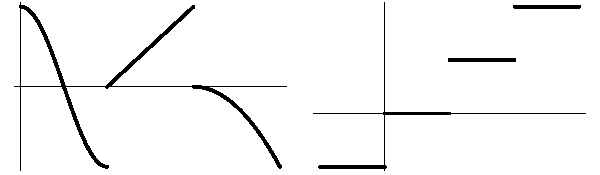
\includegraphics[width=0.6\textwidth]{calculus/differential/pwcont}
  \end{center}
  \caption{Piecewise continuous functions.}
  \label{pwcont}
\end{figure}





\paragraph{Uniform Continuity.}
\index{uniform continuity}
\index{continuity!uniform}
Consider a function $f(x)$ that is continuous on an interval.  This means 
that for any point $\xi$ in the interval and any positive $\epsilon$ there
exists a $\delta > 0$ such that $| f(x) - f(\xi) | < \epsilon$ for all
$0 < | x - \xi | < \delta$.  In general, this value of $\delta$ depends on 
both $\xi$ and $\epsilon$.  If $\delta$ can be chosen so it is a function
of $\epsilon$ alone and independent of $\xi$ then the function is said to
be \textit{uniformly continuous} on the interval.  A sufficient condition
for uniform continuity is that the function is continuous on a closed interval.






%%=============================================================================
\section{The Derivative}


Consider a function $y(x)$ on the interval $(x \ldots x+\Delta x)$
for some $\Delta x > 0$.
We define the increment $\Delta y = y(x + \Delta x) - y(x)$.  
The \textit{average rate of change}, (average velocity), of the function on the
interval is $\frac{\Delta y}{\Delta x}$.  The average rate of change 
is the slope of the secant line that passes through the points 
$(x, y(x))$ and $(x + \Delta x, y(x + \Delta x) )$.  
See Figure~\ref{increment}.


\begin{figure}[h!]
  \begin{center}
    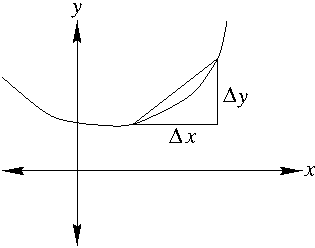
\includegraphics[width=0.33\textwidth]{calculus/differential/increment}
  \end{center}
  \caption{The increments.}
  \label{increment}
\end{figure}



If the slope of the secant line has a limit as $\Delta x$ approaches
zero then we call this slope 
the \textit{derivative} or \textit{instantaneous rate of change} 
of the function at the point $x$.  We denote the derivative by
$\frac{\dd y}{\dd x}$, which is a nice notation as the derivative is the limit 
of $\frac{\Delta y}{\Delta x}$ as $\Delta x \to 0$.
\[
\frac{\dd y}{\dd x} \equiv \lim_{\Delta x \to 0} \frac{y(x + \Delta x) - y(x)}{\Delta x}.
\]
$\Delta x$ may approach zero from below or above.
It is common to denote the derivative $\frac{\dd y}{\dd x}$ by 
$\frac{\dd }{\dd x} y$, $y'(x)$, $y'$ or $D y$.

A function is said to be \textit{differentiable} at a point if the
derivative exists there.  Note that differentiability implies continuity,
but not vice versa.





\begin{Example}
  Consider the derivative of $y(x) = x^2$ at the point $x = 1$.
  \begin{align*}
    y'(1)   &\equiv \lim_{\Delta x \to 0} 
    \frac{y(1 + \Delta x) - y(1) }{ \Delta x } \\
    &= \lim_{\Delta x \to 0} \frac{(1 + \Delta x)^2 - 1}{\Delta x} \\
    &= \lim_{\Delta x \to 0} ( 2 + \Delta x ) \\
    &= 2
  \end{align*}
  Figure~\ref{secantx2} shows the secant lines approaching the tangent line
  as $\Delta x$ approaches zero from above and below.
  \begin{figure}[h!]
    \begin{center}
      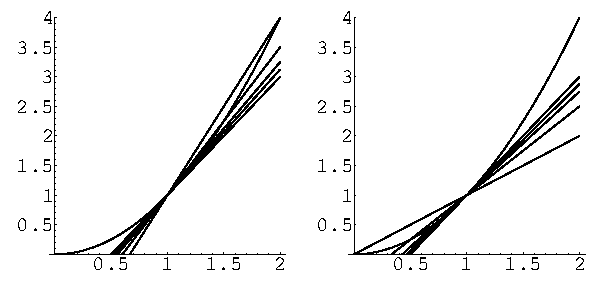
\includegraphics[width=0.8\textwidth]{calculus/differential/secantx2}
    \end{center}
    \caption{Secant lines and the tangent.}
    \label{secantx2}
  \end{figure}
\end{Example}





\begin{Example}
  We can compute the derivative of $y(x) = x^2$ at an arbitrary point $x$.
  \begin{align*}
    \frac{\dd}{\dd x} \left[ x^2 \right]
    &= \lim_{\Delta x \to 0} \frac{(x + \Delta x)^2 - x^2 }{\Delta x} \\
    &= \lim_{\Delta x \to 0} (2 x + \Delta x) \\
    &= 2 x
  \end{align*}
\end{Example}







\paragraph{Properties.}
Let $u(x)$ and $v(x)$ be differentiable.  Let $a$ and $b$ be constants.
Some fundamental properties of derivatives are:
\begin{alignat*}{2}
  &\frac{\dd}{\dd x}(a u+b v) = a \frac{\dd u}{\dd x} + b \frac{\dd v}{\dd x} 
  &\qquad &\mathrm{Linearity} 
  \\
  &\frac{\dd}{\dd x}(u v) = \frac{\dd u}{\dd x} v + u \frac{\dd v}{\dd x} 
  &\qquad &\mathrm{Product Rule} 
  \\
  &\frac{\dd}{\dd x}\left( \frac{u}{v} \right)
  = \frac{v \frac{\dd u}{\dd x} - u \frac{\dd v}{\dd x}}{v^2} 
  &\qquad &\mathrm{Quotient Rule} 
  \\
  &\frac{\dd}{\dd x}(u^a) = a u^{a-1} \frac{\dd u}{\dd x} 
  &\qquad &\mathrm{Power Rule} 
  \\
  &\frac{\dd}{\dd x} (u(v(x))) = \frac{\dd u}{\dd v} \frac{\dd v}{\dd x} 
  = u'(v(x)) v'(x)
  &\qquad &\mathrm{Chain Rule}
\end{alignat*}
These can be proved by using the definition of differentiation.


\begin{Example}
  Prove the quotient rule for derivatives.
  \begin{align*}
    \frac{\dd}{\dd x} \left( \frac{u}{v} \right)
    &= \lim_{\Delta x \to 0} \frac{\frac{u(x+\Delta x)}{v(x+\Delta x)} - \frac{u(x)}{v(x)} }{\Delta x}
    \\
    &= \lim_{\Delta x \to 0} \frac{ u(x+\Delta x) v(x) - u(x) v(x+\Delta x) }
    { \Delta x v(x) v(x + \Delta x) }
    \\
    &= \lim_{\Delta x \to 0} \frac{ u(x+\Delta x) v(x) -u(x) v(x)
      - u(x) v(x+\Delta x) + u(x) v(x) }{ \Delta x v(x) v(x) }
    \\
    &= \lim_{\Delta x \to 0} \frac{ (u(x+\Delta x) -u(x)) v(x)
      - u(x) ( v(x+\Delta x) - v(x) ) }{ \Delta x v^2(x) }
    \\
    &= \frac{ \lim_{\Delta x \to 0} \frac{u(x+\Delta x) -u(x)}{\Delta x} 
      v(x) - u(x) \lim_{\Delta x \to 0} \frac{v(x+\Delta x) - v(x)} {\Delta x}  }{ v^2(x) }
    \\
    &= \frac{v \frac{\dd u}{\dd x} - u \frac{\dd v}{\dd x}}{v^2} 
  \end{align*}
\end{Example}



\paragraph{Trigonometric Functions.}
Some derivatives of trigonometric functions are:
\begin{alignat*}{2}
  &\frac{\dd}{\dd x} \sin x = \cos x &\qquad 
  &\frac{\dd}{\dd x} \arcsin x = \frac{1}{(1-x^2)^{1/2}} 
  \\
  &\frac{\dd}{\dd x} \cos x = - \sin x &\qquad
  &\frac{\dd}{\dd x} \arccos x = \frac{-1}{(1-x^2)^{1/2}}
  \\
  &\frac{\dd}{\dd x} \tan x = \frac{1}{\cos^2 x} &\qquad
  &\frac{\dd}{\dd x} \arctan x = \frac{1}{1+x^2} 
  \\
  &\frac{\dd}{\dd x} \e^x = \e^x &\qquad 
  &\frac{\dd}{\dd x} \ln x = \frac{1}{x} 
  \\
  &\frac{\dd}{\dd x} \sinh x = \cosh x &\qquad
  &\frac{\dd}{\dd x} \arcsinh x = \frac{1}{(x^2+1)^{1/2}} 
  \\
  &\frac{\dd}{\dd x} \cosh x = \sinh x &\qquad
  &\frac{\dd}{\dd x} \arccosh x = \frac{1}{(x^2-1)^{1/2}} 
  \\
  &\frac{\dd}{\dd x} \tanh x = \frac{1}{\cosh^2 x} &\qquad
  &\frac{\dd}{\dd x} \arctanh x = \frac{1}{1-x^2} 
\end{alignat*}





\begin{Example}
  We can evaluate the derivative of $x^x$ by using the identity
  $a^b = \e^{b \ln a}$.
  \begin{align*}
    \frac{\dd}{\dd x} x^x
    &= \frac{\dd}{\dd x} \e^{x \ln x} 
    \\
    &= \e^{x \ln x} \frac{\dd}{\dd x} (x \ln x) 
    \\
    &= x^x (1 \cdot \ln x + x \frac{1}{x} ) 
    \\
    &= x^x (1 + \ln x)
  \end{align*}
\end{Example}




\paragraph{Inverse Functions.}
If we have a function $y(x)$, we can consider $x$ as a function of $y$, $x(y)$.
For example, if $y(x) = 8 x^3$ then $x(y) = \sqrt[3]{y} / 2$; if 
$y(x) = \frac{x+2}{x+1}$ then $x(y) = \frac{2-y}{y-1}$.  The derivative
of an inverse function is
\[
\frac{\dd}{\dd y} x(y) = \frac{1}{\frac{\dd y}{\dd x}}.
\]


\begin{Example}
  The inverse function of $y(x) = \e^x$ is $x(y) = \ln y$.  We can obtain
  the derivative of the logarithm from the derivative of the exponential.
  The derivative of the exponential is
  \[
  \frac{\dd y}{\dd x} = \e^x.
  \]
  Thus the derivative of the logarithm is
  \[
  \frac{\dd}{\dd y} \ln y = \frac{\dd}{\dd y} x(y) 
  = \frac{1}{\frac{\dd y}{\dd x} }
  = \frac{1}{\e^x} = \frac{1}{y}.
  \] 
\end{Example}











%%=============================================================================
\section{Implicit Differentiation}

An \textit{explicitly defined} function has the form $y = f(x)$.  A
\textit{implicitly defined} function has the form $f(x, y) = 0$.  A few 
examples of implicit functions are $x^2 + y^2 - 1 = 0$ and 
$x + y + \sin(x y) = 0$.  Often it is not possible to write an implicit
equation in explicit form.  This is true of the latter example above.
One can calculate the derivative of $y(x)$ in terms of $x$ and $y$ 
even when $y(x)$ is defined by an implicit equation.  


\begin{Example}
  Consider the implicit equation
  \[
  x^2 - x y - y^2 = 1.
  \]
  This implicit equation can be solved for the dependent variable.
  \[
  y(x) = \frac{1}{2} \left( -x \pm \sqrt{5 x^2 - 4} \right).
  \]
  We can differentiate this expression to obtain
  \[
  y' = \frac{1}{2} \left( -1 \pm \frac{5 x}{\sqrt{5 x^2 - 4}} \right).
  \]
  One can obtain the same result without first solving for $y$.  If we 
  differentiate the implicit equation, we obtain
  \[
  2 x - y - x \frac{\dd y}{\dd x} - 2 y \frac{\dd y}{\dd x} = 0.
  \]
  We can solve this equation for $\frac{\dd y}{\dd x}$.
  \[
  \frac{\dd y}{\dd x} = \frac{2x - y}{x + 2y}
  \]
  We can differentiate this expression to obtain the second derivative of $y$.
  \begin{align*}
    \frac{\dd^2 y}{\dd x^2}
    &= \frac{ (x+2y) (2-y') - (2x-y)(1+2y') }{ (x + 2y)^2 } \\
    &= \frac{ 5(y - x y') }{ (x + 2y)^2 } \\
    \intertext{Substitute in the expression for $y'$.}
    &= - \frac{ 10 (x^2 - x y - y^2) }{ (x + 2y)^2 } \\
    \intertext{Use the original implicit equation.}
    &= - \frac{ 10 }{ (x + 2y)^2 } 
  \end{align*}
\end{Example}








%%=============================================================================
\section{Maxima and Minima}

A differentiable function is \textit{increasing} where $f'(x) > 0$, 
\textit{decreasing} where $f'(x) < 0$ and \textit{stationary}
where $f'(x) = 0$.

A function $f(x)$ has a \textit{relative maxima} at a point $x = \xi$ if
there exists a neighborhood around $\xi$ such that $f(x) \leq f(\xi)$ for 
$x \in (x - \delta, x + \delta)$, $\delta > 0$.  The \textit{relative 
  minima} is defined analogously.  Note that this definition does not 
require that the function be differentiable, or even continuous.
We refer to relative maxima and minima collectively are \textit{relative
  extrema}.



\paragraph{Relative Extrema and Stationary Points.}
If $f(x)$ is differentiable and $f(\xi)$ is a relative extrema then
$x=\xi$ is a stationary point, $f'(\xi) = 0$.  We can prove this
using left and right limits.  Assume that $f(\xi)$ is a relative maxima.
Then there is a neighborhood $(x - \delta, x + \delta)$, $\delta > 0$ for 
which $f(x) \leq f(\xi)$.  Since $f(x)$ is differentiable the derivative
at $x = \xi$,
\[
f'(\xi) = \lim_{\Delta x \to 0} \frac{f(\xi + \Delta x) - f(\xi)}{\Delta x},
\]
exists.  This in turn means that the left and right limits exist and 
are equal.  Since $f(x) \leq f(\xi)$ for $\xi-\delta < x < \xi$ the left
limit is non-positive,
\[
f'(\xi) = \lim_{\Delta x \to 0^-} \frac{ f(\xi + \Delta x) - f(\xi) }
{ \Delta x } \leq 0.
\]
Since $f(x) \leq f(\xi)$ for $\xi < x < \xi + \delta$ the right
limit is nonnegative,
\[
f'(\xi) = \lim_{\Delta x \to 0^+} \frac{ f(\xi + \Delta x) - f(\xi) }
{ \Delta x } \geq 0.
\]
Thus we have $0 \leq f'(\xi) \leq 0$ which implies that $f'(\xi) = 0$.


It is not true that all stationary points are relative extrema.  That is,
$f'(\xi) = 0$ does not imply that $x = \xi$ is an extrema.  Consider the
function $f(x) = x^3$.  $x = 0$ is a stationary point since $f'(x) = x^2$,
$f'(0) = 0$.  However, $x = 0$ is neither a relative maxima nor a 
relative minima.



It is also not true that all relative extrema are stationary points.  Consider
the function $f(x) = |x|$.  The point $x = 0$ is a relative minima, but
the derivative at that point is undefined.


\paragraph{First Derivative Test.}
Let $f(x)$ be differentiable and $f'(\xi) = 0$.
\begin{itemize}
\item
  If $f'(x)$ changes sign from positive to negative as we pass through $x = \xi$
  then the point is a relative maxima.
\item
  If $f'(x)$ changes sign from negative to positive as we pass through $x = \xi$
  then the point is a relative minima.
\item
  If $f'(x)$ is not identically zero in a neighborhood of $x = \xi$ and it 
  does not change sign as we pass through the point then $x = \xi$ is 
  not a relative extrema.
\end{itemize}



\begin{Example}
  Consider $y = x^2$ and the point $x = 0$.  The function is differentiable.
  The derivative, $y' = 2x$, vanishes at $x = 0$.  Since $y'(x)$ is negative
  for $x < 0$ and positive for $x > 0$, the point $x = 0$ is a relative 
  minima.  See Figure~\ref{maxminno}.
\end{Example}





\begin{Example}
  Consider $y = \cos x$ and the point $x = 0$.  The function is differentiable.
  The derivative, $y' = - \sin x$ is positive for $-\pi < x < 0$ and negative
  for $0 < x < \pi$.  Since the sign of $y'$ goes from positive to negative,
  $x = 0$ is a relative maxima.  See Figure~\ref{maxminno}.
\end{Example}




\begin{Example}
  Consider $y = x^3$ and the point $x = 0$.  The function is differentiable.
  The derivative, $y' = 3 x^2$ is positive for $x < 0$ and positive
  for $0 < x$.  Since $y'$ is not identically zero and the sign of $y'$ 
  does not change, $x = 0$ is not a relative extrema.  See Figure~\ref{maxminno}.
\end{Example}


\begin{figure}[h!]
  \begin{center}
    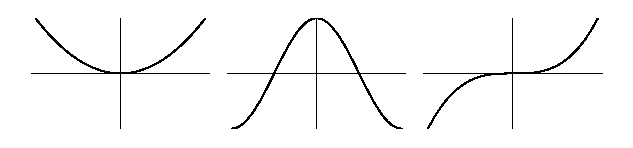
\includegraphics[width=0.8\textwidth]{calculus/differential/minmaxno}
  \end{center}
  \caption{Graphs of functions with stationary points.}
  \label{maxminno}
\end{figure}




\paragraph{Concavity.}
If the portion of a curve in some neighborhood of a point lies above the
tangent line through that point, the curve is said to be \textit{concave
  upward}.  If it lies below the tangent it is \textit{concave downward}.
If a function is twice differentiable then $f''(x) > 0$ where it is
concave upward and $f''(x) < 0$ where it is concave downward.
Note that $f''(x) > 0$ is a sufficient, but not a necessary condition
for a curve to be concave upward at a point.  A curve may be concave 
upward at a point where the second derivative vanishes.
A point where the curve changes concavity is called a \textit{point of
  inflection}.  At such a point the second derivative vanishes, 
$f''(x) = 0$.  For twice continuously differentiable functions, $f''(x) = 0$
is a necessary but not a sufficient condition for an inflection point.
The second derivative may vanish at places which are not inflection points.
See Figure~\ref{concave}.

\begin{figure}[h!]
  \begin{center}
    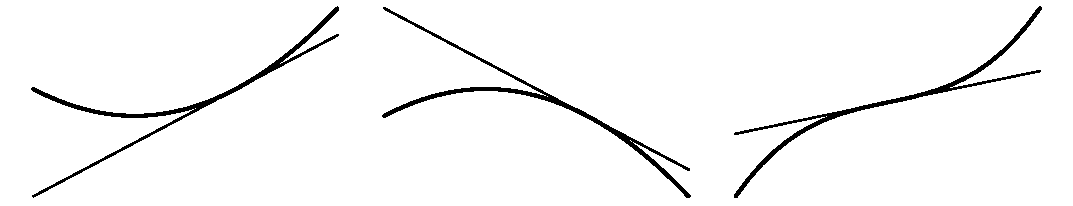
\includegraphics[width=0.8\textwidth]{calculus/differential/concave}
  \end{center}
  \caption{Concave upward, concave downward and an inflection point.}
  \label{concave}
\end{figure}






\paragraph{Second Derivative Test.}
Let $f(x)$ be twice differentiable and let $x = \xi$ be a stationary 
point, $f'(\xi) = 0$.
\begin{itemize}
\item
  If $f''(\xi) < 0$ then the point is a relative maxima.
\item
  If $f''(\xi) > 0$ then the point is a relative minima.
\item
  If $f''(\xi) = 0$ then the test fails.
\end{itemize}




\begin{Example}
  Consider the function $f(x) = \cos x$ and the point $x = 0$.  The derivatives
  of the function are $f'(x) = - \sin x$, $f''(x) = - \cos x$.  The point
  $x = 0$ is a stationary point, $f'(0) = - \sin(0) = 0$.  Since the second
  derivative is negative there, $f''(0) = - \cos(0) = -1$, the point is a 
  relative maxima.
\end{Example}






\begin{Example}
  Consider the function $f(x) = x^4$ and the point $x = 0$.  The derivatives
  of the function are $f'(x) = 4 x^3$, $f''(x) = 12 x^2$.  The point
  $x = 0$ is a stationary point.  Since the second derivative also 
  vanishes at that point the second derivative test fails.  One must use
  the first derivative test to determine that $x = 0$ is a relative minima.
\end{Example}








%%=============================================================================
\section{Mean Value Theorems}


\paragraph{Rolle's Theorem.}
If $f(x)$ is continuous in $[a,b]$, differentiable in $(a,b)$ and
$f(a) = f(b) = 0$ then there exists a point $\xi \in (a,b)$ such that
$f'(\xi) = 0$.  See Figure~\ref{rolle}.

\begin{figure}[h!]
  \begin{center}
    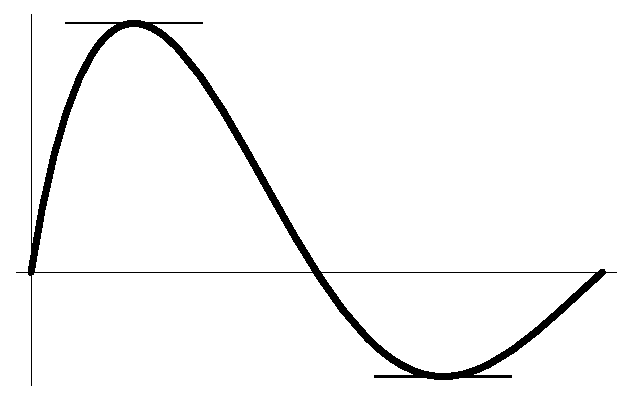
\includegraphics[width=0.3\textwidth]{calculus/differential/rolle}
  \end{center}
  \caption{Rolle's Theorem.}
  \label{rolle}
\end{figure}

To prove this we consider two cases.  First we have the 
trivial case that $f(x) \equiv 0$.  If $f(x)$ is not identically zero
then continuity implies that it must have a nonzero relative maxima or 
minima in $(a,b)$.  Let $x = \xi$ be one of these relative extrema.
Since $f(x)$ is differentiable, $x = \xi$ must be a stationary point,
$f'(\xi) = 0$.



\paragraph{Theorem of the Mean.}
If $f(x)$ is continuous in $[a,b]$ and differentiable in $(a,b)$ then there
exists a point $x = \xi$ such that
\[
f'(\xi) = \frac{f(b) - f(a)}{b - a}.
\]
That is, there is a point where the instantaneous velocity is equal to 
the average velocity on the interval.  

\begin{figure}[h!]
  \begin{center}
    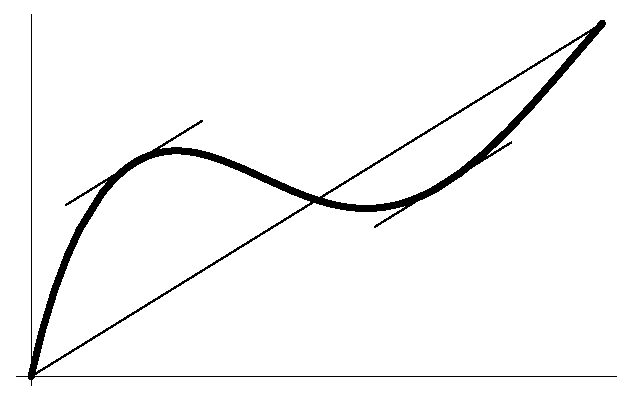
\includegraphics[width=0.3\textwidth]{calculus/differential/themean}
  \end{center}
  \caption{Theorem of the Mean.}
  \label{themean}
\end{figure}

We prove this theorem by applying
Rolle's theorem.  Consider the new function
\[
g(x) = f(x) - f(a) - \frac{f(b) - f(a)}{b - a} (x - a)
\]
Note that $g(a) = g(b) = 0$, so it satisfies the conditions of Rolle's 
theorem.  There is a point $x = \xi$ such that $g'(\xi) = 0$.
We differentiate the expression for $g(x)$ and substitute in $x = \xi$ to 
obtain the result.
\[
g'(x) = f'(x)  - \frac{f(b) - f(a)}{b-a} 
\]
\[
g'(\xi) = f'(\xi)  - \frac{f(b) - f(a)}{b-a} = 0
\]
\[
f'(\xi)  = \frac{f(b) - f(a)}{b-a}
\]




\paragraph{Generalized Theorem of the Mean.}
If $f(x)$ and $g(x)$ are continuous in $[a,b]$ and differentiable in $(a,b)$,
then there exists a point $x = \xi$ such that
\[
\frac{f'(\xi)}{g'(\xi)} = \frac{f(b) - f(a)}{g(b) - g(a)}.
\]
We have assumed that $g(a) \neq g(b)$ so that the denominator does not 
vanish and that $f'(x)$ and $g'(x)$ are not simultaneously zero which 
would produce an indeterminate form.  Note that this theorem reduces to
the regular theorem of the mean when $g(x) = x$.  The proof of the
theorem is similar to that for the theorem of the mean.





\paragraph{Taylor's Theorem of the Mean.}
If $f(x)$ is $n+1$ times continuously differentiable in $(a,b)$ then there
exists a point $x = \xi \in (a,b)$ such that
\begin{equation}
  \label{taylors_theorem}
  f(b) = f(a) + (b-a) f'(a) + \frac{(b-a)^2}{2!} f''(a) + \cdots + 
  \frac{(b-a)^n}{n!} f^{(n)}(a) 
  + \frac{(b-a)^{n+1}}{(n+1)!} f^{(n+1)}(\xi).
\end{equation}
For the case $n = 0$, the formula is
\[
f(b) = f(a) + (b-a) f'(\xi),
\]
which is just a rearrangement of the terms in the theorem of the mean,
\[
f'(\xi) = \frac{f(b) - f(a)}{b-a}.
\]
%% CONTINUE: Prove.





%%-----------------------------------------------------------------------------
\subsection{Application: Using Taylor's Theorem to Approximate Functions.}


One can use Taylor's theorem to approximate functions with polynomials.
Consider an infinitely differentiable function $f(x)$ and a point $x = a$.  
Substituting $x$ for $b$ into Equation~\ref{taylors_theorem} we obtain,
\[
\label{taylors_theorem_x}
f(x) = f(a) + (x-a) f'(a) + \frac{(x-a)^2}{2!} f''(a) + \cdots + 
\frac{(x-a)^n}{n!} f^{(n)}(a) 
+ \frac{(x-a)^{n+1}}{(n+1)!} f^{(n+1)}(\xi).
\]
If the last term in the sum is small then we can approximate our function
with an $n^{th}$ order polynomial.
\[
f(x) \approx f(a) + (x-a) f'(a) + \frac{(x-a)^2}{2!} f''(a) + \cdots + 
\frac{(x-a)^n}{n!} f^{(n)}(a) 
\]
The last term in Equation~\ref{taylors_theorem_x} is called the remainder
or the error term,
\[
R_n = \frac{(x-a)^{n+1}}{(n+1)!} f^{(n+1)}(\xi).
\]
Since the function is infinitely differentiable, $f^{(n+1)}(\xi)$ exists and
is bounded.  Therefore we note that the error must vanish as $x \to 0$ 
because of the $(x-a)^{n+1}$ factor.  We therefore suspect that our 
approximation would be a good one if $x$ is close to $a$.  Also note that
$n!$ eventually grows faster than $(x-a)^n$,
\[
\lim_{n \to \infty} \frac{(x-a)^n}{n!} = 0.
\]
So if the derivative term, $f^{(n+1)}(\xi)$, does not grow to quickly, the
error for a certain value of $x$ will get smaller with increasing $n$ and
the polynomial will become a better approximation of the function.
(It is also possible that the derivative factor grows very quickly and 
the approximation gets worse with increasing $n$.)




\begin{Example}
  Consider the function $f(x) = \e^x$.  We want a polynomial approximation of
  this function near the point $x = 0$.  Since the derivative of $\e^x$ is
  $\e^x$, the value of all the derivatives at $x = 0$ is $f^{(n)}(0) = \e^0 = 1$.
  Taylor's theorem thus states that
  \[
  \e^x = 1 + x + \frac{x^2}{2!} + \frac{x^3}{3!} + \cdots + \frac{x^n}{n!}
  + \frac{x^{n+1}}{(n+1)!} \e^\xi,
  \]
  for some $\xi \in (0,x)$.  The first few polynomial approximations of 
  the exponent about the point $x = 0$ are 
  \begin{align*}
    f_1(x) &= 1 \\
    f_2(x) &= 1 + x \\
    f_3(x) &= 1 + x + \frac{x^2}{2} \\
    f_4(x) &= 1 + x + \frac{x^2}{2} + \frac{x^3}{6} 
  \end{align*}
  The four approximations are graphed in Figure~\ref{tayexp4}.

  \begin{figure}[h!]
    \begin{center}
      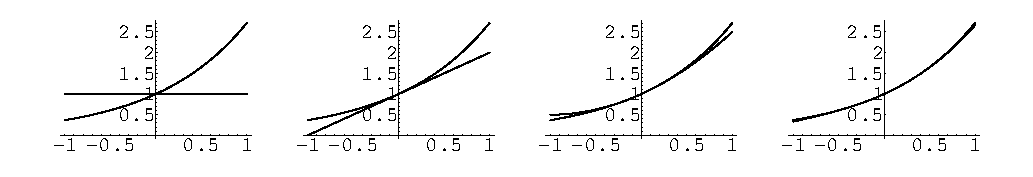
\includegraphics[width=\textwidth]{calculus/differential/tayexp4}
    \end{center}
    \caption{Four finite Taylor series approximations of the 
      exponential function.}
    \label{tayexp4}
  \end{figure}

  Note that for the range of $x$ we are looking at, the approximations
  become more accurate as the number of terms increases.
\end{Example}









\begin{Example}
  Consider the function $f(x) = \cos x$.  We want a polynomial approximation of
  this function near the point $x = 0$. The first few derivatives of $f$ are
  \begin{align*}
    f(x) &= \cos x \\
    f'(x) &= - \sin x \\
    f''(x) &= - \cos x \\
    f'''(x) &= \sin x \\
    f^{(4)}(x) &= \cos x
  \end{align*} 
  It's easy to pick out the pattern here,
  \[
  f^{(n)}(x) = 
  \begin{cases}
    (-1)^{n/2} \cos x &\mathrm{for even}\ n, \\
    (-1)^{(n+1)/2} \sin x & \mathrm{for odd}\ n.
  \end{cases}
  \]
  Since $\cos(0) = 1$ and $\sin(0) = 0$ the $n$-term approximation of the
  cosine is,
  \[
  \cos x = 1 - \frac{x^2}{2!} + \frac{x^4}{4!} - \frac{x^6}{6!} + \cdots
  + (-1)^{2(n-1)} \frac{x^{2(n-1)}}{(2(n-1))!} 
  + \frac{x^{2n}}{(2n)!} \cos \xi.
  \]
  Here are graphs of the one, two, three and four term approximations.

  \begin{figure}[h!]
    \begin{center}
      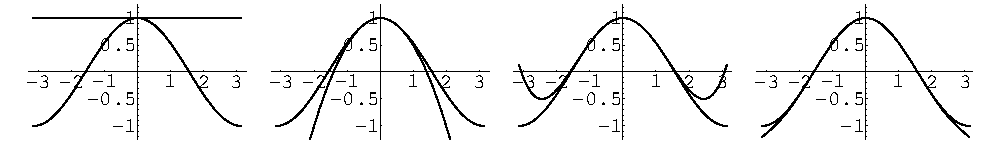
\includegraphics[width=\textwidth]{calculus/differential/taycos4}
    \end{center}
    \caption{Taylor series approximations of the cosine.}
    \label{taycos4}
  \end{figure}

  Note that for the range of $x$ we are looking at, the approximations
  become more accurate as the number of terms increases.
  Consider the ten term approximation of the cosine about $x = 0$,
  \[
  \cos x = 1 - \frac{x^2}{2!} + \frac{x^4}{4!} - \cdots - \frac{x^{18}}{18!} 
  + \frac{x^{20}}{20!} \cos \xi.
  \]
  Note that for any value of $\xi$, $|\cos \xi| \leq 1$.  Therefore the absolute
  value of the error term satisfies,
  \[
  | R | = \left| \frac{x^{20}}{20!} \cos \xi \right| \leq \frac{|x|^{20}}{20!}.
  \]
  $x^{20}/20!$ is plotted in Figure~\ref{taycoser}.

  \begin{figure}[h!]
    \begin{center}
      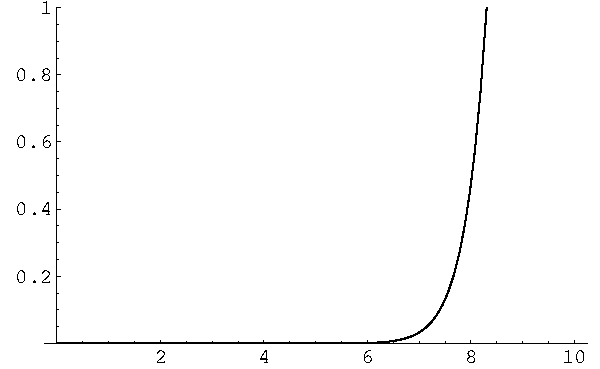
\includegraphics[width=0.3\textwidth]{calculus/differential/taycoser}
    \end{center}
    \caption{A bound on the error.}
    \label{taycoser}
  \end{figure}

  Note that the error is very small for $x < 6$, fairly small but non-negligible
  for $x \approx 7$ and large for $x > 8$.  The ten term approximation of
  the cosine, plotted below, behaves just we would predict.

  \begin{figure}[h!]
    \begin{center}
      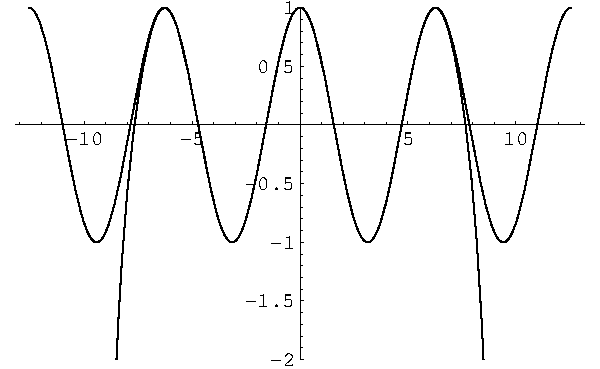
\includegraphics[width=0.3\textwidth]{calculus/differential/taycos10}
    \end{center}
    \caption{Ten term Taylor series approximation of the cosine.}
    \label{taycos10}
  \end{figure}

  The error is very small until it becomes non-negligible at $x \approx 7$
  and large at $x \approx 8$.
\end{Example}





\begin{Example}
  Consider the function $f(x) = \ln x$.  We want a polynomial approximation of
  this function near the point $x = 1$. The first few derivatives of $f$ are
  \begin{align*}
    f(x) &= \ln x \\
    f'(x) &= \frac{1}{x} \\
    f''(x) &= - \frac{1}{x^2} \\
    f'''(x) &= \frac{2}{x^3} \\
    f^{(4)}(x) &= - \frac{3}{x^4}
  \end{align*}
  The derivatives evaluated at $x = 1$ are
  \[
  f(0) = 0, \qquad f^{(n)}(0) = (-1)^{n-1} (n-1)!,\ \mathrm{for}\ n \geq 1.
  \]
  By Taylor's theorem of the mean we have,
  \[
  \ln x = (x-1) - \frac{(x-1)^2}{2} + \frac{(x-1)^3}{3} - \frac{(x-1)^4}{4}
  + \cdots + (-1)^{n-1} \frac{(x-1)^n}{n} 
  + (-1)^n \frac{(x-1)^{n+1}}{n+1} \frac{1}{\xi^{n+1}}.
  \]
  Below are plots of the 2, 4, 10 and 50 term approximations.  

  \begin{figure}[h!]
    \begin{center}
      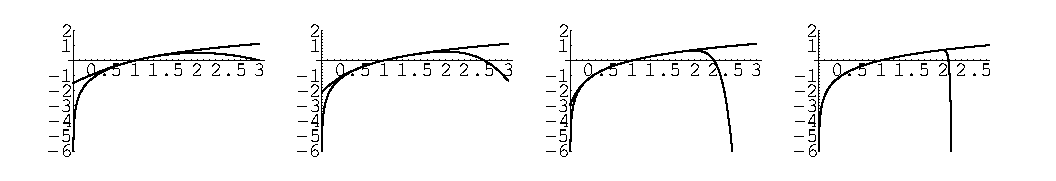
\includegraphics[width=\textwidth]{calculus/differential/taylnt4}
    \end{center}
    \caption{The 2, 4, 10 and 50 term approximations of the logarithm.}
    \label{taylnt4}
  \end{figure}

  Note that the 
  approximation gets better on the interval $(0,2)$ and worse outside this
  interval as the number of terms increases.  The Taylor series converges to
  $\ln x$ only on this interval.
\end{Example}






%%-----------------------------------------------------------------------------
\subsection{Application: Finite Difference Schemes}



\begin{Example}
  Suppose you sample a function at the discrete points $n \Delta x$, 
  $n \in \setZ$.  In Figure~\ref{sindata} we sample the function 
  $f(x) = \sin x$ on the interval $[-4,4]$ with $\Delta x = 1/4$ and 
  plot the data points.  

  \begin{figure}[h!]
    \begin{center}
      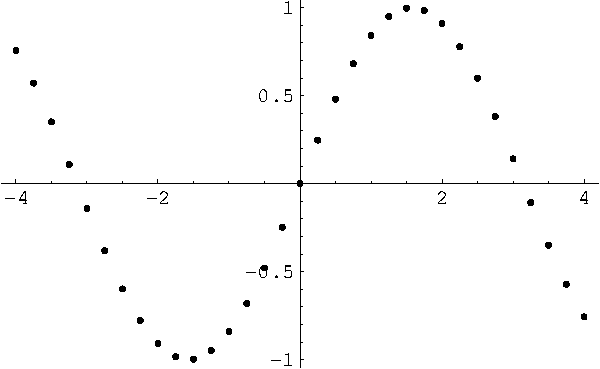
\includegraphics[width=0.4\textwidth]{calculus/differential/sindata}
    \end{center}
    \caption{Sampling of the sine function.}
    \label{sindata}
  \end{figure}

  We wish to approximate the derivative of the function on the grid points
  using only the value of the function on those discrete points.  From
  the definition of the derivative, one is lead to the formula
  \begin{equation}
    \label{first_order_scheme}
    f'(x) \approx \frac{f(x+\Delta x) - f(x)}{\Delta x}.
  \end{equation}
  Taylor's theorem states that
  \[
  f(x + \Delta x) = f(x) + \Delta x f'(x) + \frac{\Delta x^2}{2} f''(\xi).
  \]
  Substituting this expression into our formula for approximating the derivative
  we obtain
  \[
  \frac{f(x+\Delta x) - f(x)}{\Delta x} = \frac{f(x) + \Delta x f'(x)
    + \frac{\Delta x^2}{2} f''(\xi) - f(x) }{\Delta x}
  = f'(x) + \frac{\Delta x}{2} f''(\xi).
  \]
  Thus we see that the error in our approximation of the first derivative is
  $\frac{\Delta x}{2} f''(\xi)$.  Since the error has a linear factor of 
  $\Delta x$, we call this a first order accurate method.  Equation
  ~\ref{first_order_scheme} is called the \textit{forward difference 
    scheme} for calculating the first derivative.  Figure~\ref{fwdsin} shows 
  a plot of the value of this scheme for the function $f(x) = \sin x$ and 
  $\Delta x = 1/4$.  The first derivative of the function $f'(x) = \cos x$ 
  is shown for comparison.

  \begin{figure}[h!]
    \begin{center}
      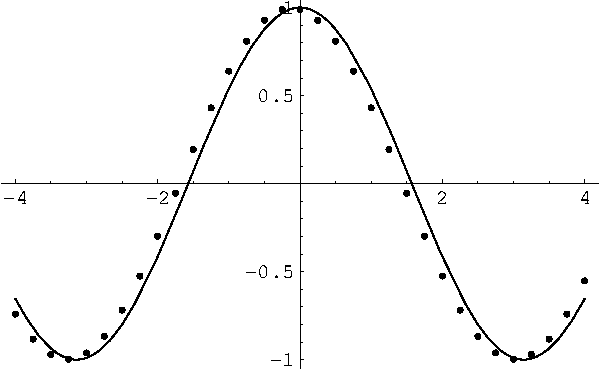
\includegraphics[width=0.4\textwidth]{calculus/differential/fwdsin}
    \end{center}
    \caption{The forward difference scheme approximation of the derivative.}
    \label{fwdsin}
  \end{figure}

  Another scheme for approximating the first derivative is the 
  \textit{centered difference scheme},
  \[
  f'(x) \approx \frac{f(x+\Delta x) - f(x-\Delta x)}{2 \Delta x}.
  \]
  Expanding the numerator using Taylor's theorem,
  \begin{align*}
    &\frac{f(x+\Delta x) - f(x-\Delta x)}{2 \Delta x} \\
    &\qquad= \frac{f(x) + \Delta x f'(x) + \frac{\Delta x^2}{2} f''(x)
      + \frac{\Delta x^3}{6} f'''(\xi)
      - f(x) + \Delta x f'(x) - \frac{\Delta x^2}{2} f''(x)
      + \frac{\Delta x^3}{6} f'''(\psi) }{2 \Delta x} \\
    &\qquad= f'(x) + \frac{\Delta x^2}{12}(f'''(\xi) + f'''(\psi)).
  \end{align*}
  The error in the approximation is quadratic in $\Delta x$.  Therefore
  this is a second order accurate scheme.
  Below is a plot of the derivative of the function and the 
  value of this scheme for the function $f(x) = \sin x$ and $\Delta x = 1/4$.

  \begin{figure}[h!]
    \begin{center}
      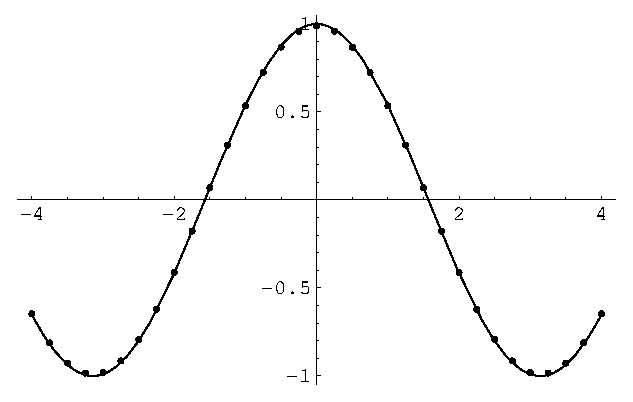
\includegraphics[width=0.4\textwidth]{calculus/differential/ctrsin}
    \end{center}
    \caption{Centered difference scheme approximation of the derivative.}
    \label{ctrsin}
  \end{figure}

  Notice how the centered difference scheme gives a better approximation of the 
  derivative than the forward difference scheme.
\end{Example}







%%=============================================================================
\section{L'Hospital's Rule}
\index{L'Hospital's rule}

Some singularities are easy to diagnose.  Consider the function 
$\frac{\cos x}{x}$ at the point $x = 0$.  The function evaluates to 
$\frac{1}{0}$ and is thus discontinuous at that point.  Since the numerator
and denominator are continuous functions and the denominator vanishes while
the numerator does not, the left and right limits as $x \to 0$ do not 
exist.  Thus the function has an infinite discontinuity at the point
$x = 0$.  More generally, a function which is composed of continuous
functions and evaluates to $\frac{a}{0}$ at a point where $a \neq 0$ must
have an infinite discontinuity there.

Other singularities require more analysis to diagnose.  Consider the 
functions $\frac{\sin x}{x}$, $\frac{\sin x}{|x|}$ and 
$\frac{\sin x}{1 - \cos x}$ at the point $x = 0$.  All three functions
evaluate to $\frac{0}{0}$ at that point, but have different kinds
of singularities.  The first has a removable discontinuity, the second has
a finite discontinuity and the third has an infinite discontinuity.
See Figure~\ref{disc3}.

\begin{figure}[h!]
  \begin{center}
    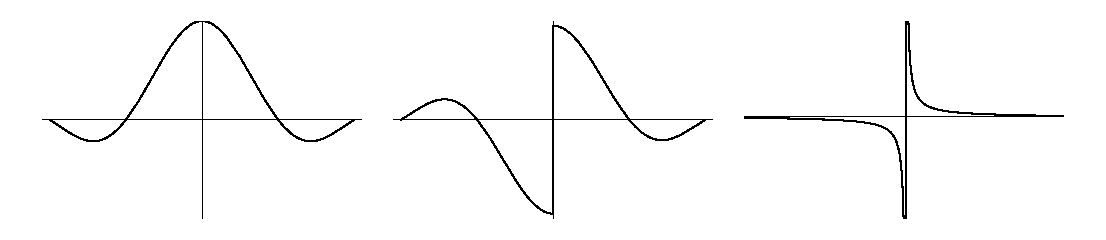
\includegraphics[width=\textwidth]{calculus/differential/disc3}
  \end{center}
  \caption{Different kinds of singularities.}
  \label{disc3}
\end{figure}



An expression that evaluates to $\frac{0}{0}$, $\frac{\infty}{\infty}$,
$0 \cdot \infty$, $\infty - \infty$, $1^\infty$, $0^0$ or $\infty^0$
is called an \textit{indeterminate}.  A function $f(x)$ which is indeterminate
at the point $x = \xi$ is singular at that point.  The singularity may be a 
removable discontinuity, a finite discontinuity or an infinite discontinuity
depending on the behavior of the function around that point.  If
$\lim_{x \to \xi} f(x)$ exists, then the function has a removable 
discontinuity.  If the limit does not exist, but the left and right limits 
do exist, then the function has a finite discontinuity.  If either the
left or right limit does not exist then the function has an infinite
discontinuity.





\paragraph{L'Hospital's Rule.}
Let $f(x)$ and $g(x)$ be differentiable and $f(\xi) = g(\xi) = 0$.  
Further, let $g(x)$ be nonzero in a deleted neighborhood of $x= \xi$, 
($g(x) \neq 0$ for $x \in 0 < |x - \xi| < \delta$).  Then
\[
\lim_{x \to \xi} \frac{f(x)}{g(x)} = \lim_{x \to \xi} \frac{f'(x)}{g'(x)}.
\]
To prove this, we note that $f(\xi) = g(\xi) = 0$ and apply the generalized
theorem of the mean.  Note that
\[
\frac{f(x)}{g(x)} = \frac{f(x) - f(\xi)}{g(x) - g(\xi)}
= \frac{f'(\psi)}{g'(\psi)}
\]
for some $\psi$ between $\xi$ and $x$.  Thus
\[
\lim_{x \to \xi} \frac{f(x)}{g(x)} 
= \lim_{\psi \to \xi} \frac{f'(\psi)}{g'(\psi)}
= \lim_{x \to \xi} \frac{f'(x)}{g'(x)}
\]
provided that the limits exist.

L'Hospital's Rule is also applicable when both functions tend to infinity
instead of zero or when the limit point, $\xi$, is at infinity.  It 
is also valid for one-sided limits.



L'Hospital's rule is directly applicable to the indeterminate forms
$\frac{0}{0}$ and $\frac{\infty}{\infty}$.


\begin{Example}
  Consider the three functions $\frac{\sin x}{x}$, $\frac{\sin x}{|x|}$ and
  $\frac{\sin x}{1 - \cos x}$ at the point $x = 0$.
  \[
  \lim_{x \to 0} \frac{\sin x}{x}
  = \lim_{x \to 0} \frac{\cos x}{1} 
  = 1
  \]
  Thus $\frac{\sin x}{x}$ has a removable discontinuity at $x = 0$.
  \[
  \lim_{x \to 0^+} \frac{\sin x}{|x|}
  = \lim_{x \to 0^+} \frac{\sin x}{x} = 1
  \]
  \[
  \lim_{x \to 0^-} \frac{\sin x}{|x|}
  = \lim_{x \to 0^-} \frac{\sin x}{-x} = -1
  \]
  Thus $\frac{\sin x}{|x|}$ has a finite discontinuity at $x = 0$.
  \[
  \lim_{x \to 0} \frac{\sin x}{1 - \cos x}
  = \lim_{x \to 0} \frac{\cos x}{\sin x}
  = \frac{1}{0} = \infty
  \]
  Thus $\frac{\sin x}{1 - \cos x}$ has an infinite discontinuity at $x = 0$.
\end{Example}




\begin{Example}
  Let $a$ and $d$ be nonzero.
  \begin{align*}
    \lim_{x \to \infty} \frac{a x^2 + b x + c}{d x^2 + e x + f}
    &= \lim_{x \to \infty} \frac{2 a x + b}{2 d x + e} \\
    &= \lim_{x \to \infty} \frac{2 a}{2 d} \\
    &= \frac{a}{d}
  \end{align*}
\end{Example}





\begin{Example}
  Consider
  \[
  \lim_{x \to 0} \frac{\cos x - 1}{x \sin x}.
  \]
  This limit is an indeterminate of the form $\frac{0}{0}$.  Applying
  L'Hospital's rule we see that limit is equal to
  \[
  \lim_{x \to 0} \frac{-\sin x}{x \cos x + \sin x}.
  \]
  This limit is again an indeterminate of the form $\frac{0}{0}$.  We apply
  L'Hospital's rule again.
  \[
  \lim_{x \to 0} \frac{- \cos x}{ - x \sin x + 2 \cos x } = - \frac{1}{2}
  \]
  Thus the value of the original limit is $- \frac{1}{2}$.  We could also
  obtain this result by expanding the functions in Taylor series.
  \begin{align*}
    \lim_{x \to 0} \frac{\cos x - 1}{x \sin x}
    &= \lim_{x \to 0} \frac{\left( 1 - \frac{x^2}{2} + \frac{x^4}{24} 
        - \cdots \right) - 1 }{ x \left( x - \frac{x^3}{6} 
        + \frac{x^5}{120} - \cdots \right)} \\
    &= \lim_{x \to 0} \frac{- \frac{x^2}{2} + \frac{x^4}{24} - \cdots }
    { x^2 - \frac{x^4}{6} + \frac{x^6}{120} - \cdots } \\
    &= \lim_{x \to 0} \frac{- \frac{1}{2} + \frac{x^2}{24} - \cdots }
    { 1 - \frac{x^2}{6} + \frac{x^4}{120} - \cdots } \\
    &= - \frac{1}{2}
  \end{align*}
\end{Example}




We can apply L'Hospital's Rule to the indeterminate forms $0 \cdot \infty$
and $\infty - \infty$ by rewriting the expression in a different form, 
(perhaps putting the expression over a common denominator).  If at first
you don't succeed, try, try again.  You may have to apply L'Hospital's 
rule several times to evaluate a limit.


\begin{Example}
  \begin{align*}
    \lim_{x \to 0} \left( \cot x - \frac{1}{x} \right)
    &= \lim_{x \to 0} \frac{x \cos x - \sin x}{x \sin x} \\
    &= \lim_{x \to 0} \frac{\cos x - x \sin x - \cos x}
    {\sin x + x \cos x} \\
    &= \lim_{x \to 0} \frac{- x \sin x } {\sin x + x \cos x} \\
    &= \lim_{x \to 0} \frac{- x \cos x - \sin x } 
    {\cos x + \cos x - x \sin x } \\
    &= 0
  \end{align*}
\end{Example}


You can apply L'Hospital's rule to the indeterminate forms $1^\infty$, 
$0^0$ or $\infty^0$ by taking the logarithm of the expression.


\begin{Example}
  Consider the limit,
  \[
  \lim_{x \to 0} x^x,
  \]
  which gives us the indeterminate form $0^0$.
  The logarithm of the expression is
  \[
  \ln( x^x ) = x \ln x.
  \]
  As $x \to 0$ we now have the indeterminate form $0 \cdot \infty$.  By 
  rewriting the expression, we can apply L'Hospital's rule.
  \begin{align*}
    \lim_{x \to 0} \frac{\ln x}{1/x}
    &= \lim_{x \to 0} \frac{1/x}{-1/x^2} \\
    &= \lim_{x \to 0} (-x) \\
    &= 0
  \end{align*}
  Thus the original limit is
  \[
  \lim_{x \to 0} x^x = \e^0 = 1.
  \]
\end{Example}









\raggedbottom
%%============================================================================
\pagebreak
\flushbottom
\section{Exercises}


%%-----------------------------------------------------------------------------
\begin{large}
  \noindent
  \textbf{Limits of Functions}
\end{large}


\begin{Exercise}[mathematica/calculus/differential/limits.nb]
  \label{exercise lim sin 1/x}
  Does 
  \[
  \lim_{x \to 0} \sin \left( \frac{1}{x} \right)
  \]
  exist?

  \hintsolution{lim sin 1/x}
\end{Exercise}







\begin{Exercise}[mathematica/calculus/differential/limits.nb]
  \label{exercise lim x sin 1/x}
  Does 
  \[
  \lim_{x \to 0} x \sin \left( \frac{1}{x} \right)
  \]
  exist?

  \hintsolution{lim x sin 1/x}
\end{Exercise}


\begin{Exercise}[mathematica/calculus/differential/limits.nb]
  \label{exercise limit sqrt n 5}
  Evaluate the limit:
  \[
  \lim_{n \to \infty} \sqrt[n]{5}.
  \]

  \hintsolution{limit sqrt n 5}
\end{Exercise}



%%-----------------------------------------------------------------------------
\begin{large}
  \noindent
  \textbf{Continuous Functions}
\end{large}



\begin{Exercise}
  \label{exercise sin 1/x continuous}
  Is the function $\sin(1/x)$ continuous in the open interval $(0,1)$?
  Is there a value of $a$ such that the function defined by
  \[
  f(x) =
  \begin{cases}
    \sin(1/x) &\mathrm{for}\ x \neq 0, \\
    a &\mathrm{for}\ x = 0
  \end{cases}
  \]
  is continuous on the closed interval $[0,1]$?

  \hintsolution{sin 1/x continuous}
\end{Exercise}

%%
\begin{Exercise}
  \label{exercise sin 1/x uniformly continuous}
  Is the function $\sin(1/x)$ uniformly continuous in the open interval $(0,1)$?

  \hintsolution{sin 1/x uniformly continuous}
\end{Exercise}


%%
\begin{Exercise}
  \label{exercise sqrt x uniformly continuous}
  Are the functions $\sqrt{x}$ and $\frac{1}{x}$ uniformly continuous on 
  the interval $(0,1)$?

  \hintsolution{sqrt x uniformly continuous}
\end{Exercise}



\begin{Exercise}
  \label{exercise continuous closed uniformly}
  Prove that a function which is continuous on a closed interval is
  uniformly continuous on that interval.

  \hintsolution{continuous closed uniformly}
\end{Exercise}







\begin{Exercise}
  \label{exercise lim a = L lim a2 = L2}
  Prove or disprove each of the following.
  \begin{enumerate}
  \item 
    If $\lim_{n \to \infty} a_n = L$ then $\lim_{n \to \infty} a_n^2 = L^2$.
  \item 
    If $\lim_{n \to \infty} a_n^2 = L^2$ then $\lim_{n \to \infty} a_n = L$.
  \item 
    If $a_n > 0$ for all $n > 200$, and $\lim_{n \to \infty} a_n = L$, then $L > 0$.
  \item 
    If $f : \setR \mapsto \setR$ is continuous and $\lim_{x \to \infty} f(x) = L$, then for 
    $n \in \setZ$, $\lim_{n \to \infty} f(n) = L$.
  \item 
    If $f : \setR \mapsto \setR$ is continuous and $\lim_{n \to \infty} f(n) = L$, then for 
    $x \in \setR$, $\lim_{x \to \infty} f(x) = L$.
  \end{enumerate}

  \hintsolution{lim a = L lim a2 = L2}
\end{Exercise}







%%-----------------------------------------------------------------------------
\begin{large}
  \noindent
  \textbf{The Derivative}
\end{large}





\begin{Exercise}[mathematica/calculus/differential/derivative.nb]
  \label{exercise differentiation properties}
  Use the definition of differentiation to prove the following identities
  where $f(x)$ and $g(x)$ are differentiable functions and $n$ is a positive 
  integer.
  \begin{enumerate}
  \item
    $\frac{\dd}{\dd x} (x^n) = n x^{n-1}$, $\quad$ (I suggest that you use Newton's
    binomial formula.)
  \item
    $\frac{\dd}{\dd x} (f(x) g(x)) = f \frac{\dd g}{\dd x} 
    + g \frac{\dd f}{\dd x}$
  \item
    $\frac{\dd}{\dd x} (\sin x) = \cos x$.  (You'll need to use some 
    trigonometric identities.)
  \item
    $\frac{\dd}{\dd x} (f(g(x))) = f'(g(x)) g'(x)$
  \end{enumerate}

  \hintsolution{differentiation properties}
\end{Exercise}





\begin{Exercise}[mathematica/calculus/differential/derivative.nb]
  \label{exercise differentiable f = x|x|}
  Use the definition of differentiation to determine if the following 
  functions are differentiable at $x = 0$.
  \begin{enumerate}
  \item
    $f(x) = x |x|$
  \item
    $f(x) = \sqrt{1 + |x|}$
  \end{enumerate}

  \hintsolution{differentiable f = x|x|}
\end{Exercise}









\begin{Exercise}[mathematica/calculus/differential/derivative.nb]
  \label{exercise d/dx x sin cos x}
  Find the first derivatives of the following:
  \renewcommand{\theenumi}{\alph{enumi}}
  \begin{enumerate}
  \item
    $x \sin( \cos x)$
  \item
    $f( \cos( g(x) ) )$
  \item
    $\frac{1}{f(\ln x)}$
  \item
    $x^{x^x}$
  \item
    $|x| \sin |x|$
  \end{enumerate}
  \renewcommand{\theenumi}{\arabic{enumi}}

  \hintsolution{d/dx x sin cos x}
\end{Exercise}



\begin{Exercise}[mathematica/calculus/differential/derivative.nb]
  \label{exercise d/dx arcsin x}
  Using 
  \[
  \frac{\dd}{\dd x} \sin x = \cos x \quad \mathrm{and} \quad
  \frac{\dd}{\dd x} \tan x = \frac{1}{\cos^2 x}
  \]
  find the derivatives of $\arcsin x$ and $\arctan x$.

  \hintsolution{d/dx arcsin x}
\end{Exercise}




%%-----------------------------------------------------------------------------
\begin{large}
  \noindent
  \textbf{Implicit Differentiation}
\end{large}


\begin{Exercise}[mathematica/calculus/differential/implicit.nb]
  \label{exercise tangent circle}
  Find $y'(x)$, given that $x^2 + y^2 = 1$.  What is $y'(1/2)$?

  \hintsolution{tangent circle}
\end{Exercise}





\begin{Exercise}[mathematica/calculus/differential/implicit.nb]
  \label{exercise y' y'' circle}
  Find $y'(x)$ and $y''(x)$, given that $x^2 - x y + y^2 = 3$.
  (Write each in terms of $x$ and $y$.)

  \hintsolution{y' y'' circle}
\end{Exercise}



%%-----------------------------------------------------------------------------
\begin{large}
  \noindent
  \textbf{Maxima and Minima}
\end{large}


\begin{Exercise}[mathematica/calculus/differential/maxima.nb]
  \label{exercise max min x(12-2x)2}
  Identify any maxima and minima of the following functions.
  \renewcommand{\theenumi}{\alph{enumi}}
  \begin{enumerate}
  \item
    $\displaystyle f(x) = x(12-2x)^2$
  \item
    $\displaystyle f(x) = \sqrt[3]{(x-2)^2}$
  \end{enumerate}
  \renewcommand{\theenumi}{\arabic{enumi}}

  \hintsolution{max min x(12-2x)2}
\end{Exercise}




\begin{Exercise}[mathematica/calculus/differential/maxima.nb]
  \label{exercise surface area cup}
  A cylindrical container with a circular base and an open top is to hold
  $64 \mathrm{cm}^3$.  Find its dimensions so that the surface area of the 
  cup is a minimum.

  \hintsolution{surface area cup}
\end{Exercise}



%%-----------------------------------------------------------------------------
\begin{large}
  \noindent
  \textbf{Mean Value Theorems}
\end{large}


\begin{Exercise}
  \label{exercise generalized theorem of the mean}
  Prove the generalized theorem of the mean.  
  If $f(x)$ and $g(x)$ are continuous in $[a,b]$ and differentiable in $(a,b)$,
  then there exists a point $x = \xi$ such that
  \[
  \frac{f'(\xi)}{g'(\xi)} = \frac{f(b) - f(a)}{g(b) - g(a)}.
  \]
  Assume that $g(a) \neq g(b)$ so that the denominator does not
  vanish and that $f'(x)$ and $g'(x)$ are not simultaneously zero which
  would produce an indeterminate form.  

  \hintsolution{generalized theorem of the mean}
\end{Exercise}


\begin{Exercise}[mathematica/calculus/differential/taylor.nb]
  \label{exercise polynomial approximation sin x}
  Find a polynomial approximation of $\sin x$ on the interval $[-1,1]$ that
  has a maximum error of $\frac{1}{1000}$.  Don't use any more terms that you
  need to.  Prove the error bound.  Use your polynomial to approximate
  $\sin(1)$.

  \hintsolution{polynomial approximation sin x}
\end{Exercise}






\begin{Exercise}[mathematica/calculus/differential/taylor.nb]
  \label{exercise second difference centered}
  You use the formula $\frac{f(x+\Delta x)-2f(x)+f(x-\Delta x)}{\Delta x^2}$
  to approximate $f''(x)$.  What is the error in this approximation?

  \hintsolution{second difference centered}
\end{Exercise}



\begin{Exercise}
  \label{exercise first derivative higher}
  The formulas $\frac{f(x + \Delta x) - f(x)}{\Delta x}$ and
  $\frac{f(x + \Delta x) - f(x - \Delta x)}{2 \Delta x}$ are first and
  second order accurate schemes for approximating the first derivative
  $f'(x)$. Find a couple of other schemes that have successively higher orders
  of accuracy.  Would these higher order schemes actually give a better
  approximation of $f'(x)$?  Remember that $\Delta x$ is small, but not
  infinitesimal.

  \hintsolution{first derivative higher}
\end{Exercise}



%%-----------------------------------------------------------------------------
\begin{large}
  \noindent
  \textbf{L'Hospital's Rule}
\end{large}


\begin{Exercise}[mathematica/calculus/differential/lhospitals.nb]
  \label{exercise lim (x - sin x)/x3}
  Evaluate the following limits.
  \renewcommand{\theenumi}{\alph{enumi}}
  \begin{enumerate}
  \item
    $\lim_{x \to 0} \frac{x - \sin x}{x^3}$
  \item
    $\lim_{x \to 0} \left( \csc x - \frac{1}{x} \right)$
  \item
    $\lim_{x \to +\infty} \left( 1 + \frac{1}{x} \right)^x$
  \item
    $\lim_{x \to 0} \left( \csc^2 x - \frac{1}{x^2} \right)$.
    (First evaluate using L'Hospital's rule then using a Taylor series expansion.
    You will find that the latter method is more convenient.)
  \end{enumerate}
  \renewcommand{\theenumi}{\arabic{enumi}}

  \hintsolution{lim (x - sin x)/x3}
\end{Exercise}






\begin{Exercise}[mathematica/calculus/differential/lhospitals.nb]
  \label{exercise lim x a/x}
  Evaluate the following limits,
  \[
  \lim_{x \to \infty} x^{a/x}, \qquad
  \lim_{x \to \infty} \left( 1 + \frac{a}{x} \right)^{b x},
  \]
  where $a$ and $b$ are constants.

  \hintsolution{lim x a/x}
\end{Exercise}





%% CONTINUE: prove L'Hospital's rule at infinity.












\raggedbottom
%%=============================================================================
\pagebreak
\flushbottom
\section{Hints}


%%----------------------------------------------------------------------------
%% Limits of Functions


\begin{Hint}
  \label{hint lim sin 1/x}
  Apply the $\epsilon$, $\delta$ definition of a limit.
\end{Hint}





\begin{Hint}
  \label{hint lim x sin 1/x}
  Set $y = 1/x$.  Consider $\lim_{y \to \infty}$.
\end{Hint}


\begin{Hint}
  \label{hint limit sqrt n 5}
  Write $\sqrt[n]{5}$ in terms of the exponential function.
\end{Hint}


%%----------------------------------------------------------------------------
%% Continuous Functions



\begin{Hint}
  \label{hint sin 1/x continuous}
  The composition of continuous functions is continuous.
  Apply the definition of continuity and look at the point $x = 0$.
\end{Hint}


\begin{Hint}
  \label{hint sin 1/x uniformly continuous}
  Note that for $x_1 = \frac{1}{(n-1/2) \pi}$ and $x_2 = \frac{1}{(n+1/2) \pi}$ 
  where $n \in \setZ$ we have $| \sin(1/x_1) - \sin(1/x_2)| = 2$.  
\end{Hint}


\begin{Hint}
  \label{hint sqrt x uniformly continuous}
  Note that the function $\sqrt{x + \delta} - \sqrt{x}$ is a decreasing 
  function of $x$ and an increasing function of $\delta$ for positive $x$ 
  and $\delta$.  Bound this function for fixed $\delta$.

  Consider any positive $\delta$ and $\epsilon$.  For what values of $x$ is
  \[
  \frac{1}{x} - \frac{1}{x+\delta} > \epsilon.
  \]
\end{Hint}



\begin{Hint}
  \label{hint continuous closed uniformly}
  Let the function $f(x)$ be continuous on a closed interval.
  Consider the function 
  \[
  e(x,\delta) = \sup_{|\xi-x|<\delta} | f(\xi) - f(x) |.
  \]
  Bound $e(x,\delta)$ with a function of $\delta$ alone.
\end{Hint}








\begin{Hint}
  \label{hint lim a = L lim a2 = L2}
  CONTINUE
  \begin{enumerate}
  \item 
    If $\lim_{n \to \infty} a_n = L$ then $\lim_{n \to \infty} a_n^2 = L^2$.
  \item 
    If $\lim_{n \to \infty} a_n^2 = L^2$ then $\lim_{n \to \infty} a_n = L$.
  \item 
    If $a_n > 0$ for all $n > 200$, and $\lim_{n \to \infty} a_n = L$, then $L > 0$.
  \item 
    If $f : \setR \mapsto \setR$ is continuous and $\lim_{x \to \infty} f(x) = L$, then for 
    $n \in \setZ$, $\lim_{n \to \infty} f(n) = L$.
  \item 
    If $f : \setR \mapsto \setR$ is continuous and $\lim_{n \to \infty} f(n) = L$, then for 
    $x \in \setR$, $\lim_{x \to \infty} f(x) = L$.
  \end{enumerate}
\end{Hint}







%%-----------------------------------------------------------------------------
%% The Derivative



\begin{Hint}
  \label{hint differentiation properties}
  \renewcommand{\theenumi}{\alph{enumi}}
  \begin{enumerate}
    %%
  \item
    Newton's binomial formula is
    \[
    (a + b)^n = \sum_{k=0}^n \binom{n}{k} a^{n-k} b^k
    = a^n + a^{n-1} b + \frac{n(n-1)}{2} a^{n-2} b^2 + \cdots + n a b^{n-1}
    + b^n.
    \]
    Recall that the binomial coefficient is
    \[
    \binom{n}{k} = \frac{n!}{(n-k)! k!}.
    \]
    %%
  \item
    Note that
    \[
    \frac{\dd}{\dd x} (f(x) g(x))
    = \lim_{\Delta x \to 0} \left[ \frac{f(x+\Delta x) g(x+\Delta x)
        - f(x) g(x)} {\Delta x} \right] 
    \]
    and
    \[
    g(x) f'(x) + f(x) g'(x)
    = g(x) \lim_{\Delta x \to 0} \left[ \frac{f(x+\Delta x) - f(x)}
      {\Delta x} \right] +
    f(x) \lim_{\Delta x \to 0} \left[ \frac{g(x+\Delta x)- g(x)}
      {\Delta x} \right].
    \]
    Fill in the blank.
    %%
  \item
    First prove that
    \[
    \lim_{\theta \to 0} \frac{\sin \theta}{\theta} = 1.
    \]
    and
    \[
    \lim_{\theta \to 0} \left[ \frac{\cos \theta - 1}{\theta} \right] = 0.
    \]
    %%
  \item
    Let $u = g(x)$.
    Consider a nonzero increment $\Delta x$, which induces the increments
    $\Delta u$ and $\Delta f$.  By definition,
    \[
    \Delta f = f(u + \Delta u) - f(u), \qquad
    \Delta u = g(x + \Delta x) - g(x),
    \]
    and $\Delta f, \Delta u \to 0$ as $\Delta x \to 0$.
    If $\Delta u \neq 0$ then we have
    \[
    \epsilon = \frac{\Delta f}{\Delta u} - \frac{\dd f}{\dd u} \to 0 \quad \mathrm{as}
    \quad \Delta u \to 0.
    \]
    If $\Delta u = 0$ for some values of $\Delta x$ then $\Delta f$ also vanishes
    and we define $\epsilon = 0$ for theses values.  In either case,
    \[
    \Delta y = \frac{\dd f}{\dd u} \Delta u + \epsilon \Delta u.
    \]
    Continue from here.
  \end{enumerate}
  \renewcommand{\theenumi}{\arabic{enumi}}
\end{Hint}





\begin{Hint}
  \label{hint differentiable f = x|x|}
  %% CONTINUE
\end{Hint}



\begin{Hint}
  \label{hint d/dx x sin cos x}
  \renewcommand{\theenumi}{\alph{enumi}}
  \begin{enumerate}
    %%
  \item
    Use the product rule and the chain rule.
    %%
  \item
    Use the chain rule.
    %%
  \item
    Use the quotient rule and the chain rule.
    %%
  \item
    Use the identity $a^b = \e^{b \ln a}$.
    %%
  \item
    Use the fact that the sine is an odd function, i.e. 
    $\sin(-x) = - \sin x$.
  \end{enumerate}
  \renewcommand{\theenumi}{\arabic{enumi}}
\end{Hint}






\begin{Hint}
  \label{hint d/dx arcsin x}
  Use that $x'(y) = 1/y'(x)$ and the identities $\cos x = (1 - \sin^2 x)^{1/2}$
  and $\cos(\arctan x) = \frac{1}{(1+x^2)^{1/2}}$.
\end{Hint}











%%-----------------------------------------------------------------------------
%% Implicit Differentiation




\begin{Hint}
  \label{hint tangent circle}
  Differentiate the equation.
  \begin{gather*}
    x^2 + y^2 = 1
    \\
    2 x + 2 y y' = 0
  \end{gather*}
  Solve this equation for $y'(x)$ and write $y(x)$ in terms of $x$.
\end{Hint}






\begin{Hint}
  \label{hint y' y'' circle}
  Differentiate the equation and solve for $y'(x)$ in terms of $x$ and $y(x)$.
  Differentiate the expression for $y'(x)$ to obtain $y''(x)$.  You'll use that
  \[
  x^2 - x y + y^2 = 3.
  \]
\end{Hint}



%%-----------------------------------------------------------------------------
%% Maxima and Minima



\begin{Hint}
  \label{hint max min x(12-2x)2}
  \renewcommand{\theenumi}{\alph{enumi}}
  \begin{enumerate}
    %%
  \item
    Use the second derivative test.
    %%
  \item
    The function is not differentiable at the point $x = 2$ so you can't use
    a derivative test at that point.
  \end{enumerate}
  \renewcommand{\theenumi}{\arabic{enumi}}
\end{Hint}







\begin{Hint}
  \label{hint surface area cup}
  Let $r$ be the radius and $h$ the height of the cylinder.  The volume of
  the cup is $\pi r^2 h = 64$.  The radius and height are related by
  $h = \frac{64}{\pi r^2}$.  Write the surface area as a function of $r$ and
  use the second derivative test to find its minimum.
\end{Hint}



%%-----------------------------------------------------------------------------
%% Mean Value Theorems


\begin{Hint}
  \label{hint generalized theorem of the mean}
  The proof is analogous to the proof of the theorem of the mean.  
  Use Rolle's theorem.
\end{Hint}



\begin{Hint}
  \label{hint polynomial approximation sin x}
  The first few terms in the Taylor series of $\sin(x)$ about $x=0$ are
  \[
  \sin(x) = x - \frac{x^3}{6} + \frac{x^5}{120} - \frac{x^7}{5040}
  + \frac{x^9}{362880} + \cdots.
  \]
  When determining the error, use the fact that $|\cos x_0| \leq 1$ and
  $|x^n| \leq 1$ for $x \in [-1,1]$.
\end{Hint}




\begin{Hint}
  \label{hint second difference centered}
  The terms in the approximation have the Taylor series,
  \begin{align*}
    f(x+\Delta x) &= f(x) + \Delta x f'(x) + \frac{\Delta x^2}{2} f''(x)
    +\frac{\Delta x^3}{6} f'''(x) + \frac{\Delta x^4}{24} f''''(x_1), \\
    f(x-\Delta x) &= f(x) - \Delta x f'(x) + \frac{\Delta x^2}{2} f''(x)
    -\frac{\Delta x^3}{6} f'''(x) + \frac{\Delta x^4}{24} f''''(x_2),
  \end{align*}
  where $x \leq x_1 \leq x + \Delta x$ and $x - \Delta x \leq x_2 \leq x$.
\end{Hint}




\begin{Hint}
  \label{hint first derivative higher}
  %% CONTINUE
\end{Hint}



%%-----------------------------------------------------------------------------
%% L'Hospital's Rule





\begin{Hint}
  \label{hint lim (x - sin x)/x3}
  \renewcommand{\theenumi}{\alph{enumi}}
  \begin{enumerate}
    %%
  \item
    Apply L'Hospital's rule three times.
    %%
  \item
    You can write the expression as
    \[
    \frac{x - \sin x}{x \sin x}.
    \]
    %%
  \item
    Find the limit of the logarithm of the expression.
    %%
  \item
    It takes four successive applications of L'Hospital's rule to evaluate
    the limit.

    For the Taylor series expansion method,
    \[
    \csc^2 x - \frac{1}{x^2} 
    = \frac{x^2 - \sin^2 x}{ x^2 \sin^2 x } 
    = \frac{x^2 - (x - x^3/6 + O(x^5))^2}
    { x^2 (x + O(x^3))^2 } 
    \]
  \end{enumerate}
  \renewcommand{\theenumi}{\arabic{enumi}}
\end{Hint}







\begin{Hint}
  \label{hint lim x a/x}
  To evaluate the limits use the identity $a^b = \e^{b \ln a}$
  and then apply L'Hospital's rule.
\end{Hint}
















\raggedbottom
%%=============================================================================
\pagebreak
\flushbottom
\section{Solutions}


%%----------------------------------------------------------------------------
%% Limits of Functions


\begin{Solution}
  \label{solution lim sin 1/x}
  Note that in any open neighborhood of zero, $(-\delta,\delta)$, the 
  function $\sin(1/x)$ takes on all values in the interval $[-1,1]$.  
  Thus if we choose a positive $\epsilon$ such that $\epsilon < 1$ then there
  is no value of $\psi$ for which $| \sin(1/x) - \psi | < \epsilon$ for all
  $x \in (-\epsilon,\epsilon)$.  Thus the limit does not exist.
\end{Solution}





\begin{Solution}
  \label{solution lim x sin 1/x}
  We make the change of variables $y = 1/x$ and consider $y \to \infty$.  We use that
  $\sin(y)$ is bounded.
  \[
  \lim_{x \to 0} x \sin \left( \frac{1}{x} \right)
  = \lim_{y \to \infty} \frac{1}{y} \sin(y)
  = 0
  \]
\end{Solution}


\begin{Solution}
  \label{solution limit sqrt n 5}
  We write $\sqrt[n]{5}$ in terms of the exponential function and then
  evaluate the limit.
  \begin{align*}
    \lim_{n \to \infty} \sqrt[n]{5}
     &= \lim_{n \to \infty} \exp \left( \frac{\ln 5}{n} \right)
     \\
     &= \exp \left( \lim_{n \to \infty} \frac{\ln 5}{n} \right)
     \\
     &= \e^{0}
     \\
     &= 1
  \end{align*}
\end{Solution}




%%----------------------------------------------------------------------------
%% Continuous Functions



\begin{Solution}
  \label{solution sin 1/x continuous}
  Since $\frac{1}{x}$ is continuous in the interval $(0,1)$ and the function
  $\sin(x)$ is continuous everywhere, the composition $\sin(1/x)$ is 
  continuous in the interval $(0,1)$.

  Since $\lim_{x \to 0} \sin(1/x)$ does not exist, there is no way of defining
  $\sin(1/x)$ at $x = 0$ to produce a function that is continuous in $[0,1]$.
\end{Solution}


\begin{Solution}
  \label{solution sin 1/x uniformly continuous}
  Note that for $x_1 = \frac{1}{(n-1/2) \pi}$ and $x_2 = \frac{1}{(n+1/2) \pi}$ 
  where $n \in \setZ$ we have $| \sin(1/x_1) - \sin(1/x_2)| = 2$.  Thus 
  for any $0 < \epsilon < 2$ there is no value of $\delta > 0$ such that 
  $| \sin(1/x_1) - \sin(1/x_2)| < \epsilon$ for all $x_1, x_2 \in (0,1)$ and
  $|x_1 - x_2| < \delta$.  Thus $\sin(1/x)$ is not uniformly continuous
  in the open interval $(0,1)$.
\end{Solution}



\begin{Solution}
  \label{solution sqrt x uniformly continuous}
  First consider the function $\sqrt{x}$.  Note that the function
  $\sqrt{x + \delta} - \sqrt{x}$ is a decreasing function of $x$ 
  and an increasing function of $\delta$
  for positive $x$ and $\delta$.  Thus for any fixed $\delta$, the maximum 
  value of $\sqrt{x + \delta} - \sqrt{x}$ is bounded by $\sqrt{\delta}$.
  Therefore on the interval $(0,1)$, a sufficient condition for 
  $| \sqrt{x} - \sqrt{\xi} | < \epsilon$ is $| x - \xi | < \epsilon^2$.
  The function $\sqrt{x}$ is uniformly continuous on the interval $(0,1)$.

  Consider any positive $\delta$ and $\epsilon$.  
  Note that 
  \[
  \frac{1}{x} - \frac{1}{x+\delta} > \epsilon
  \]
  for
  \[
  x < \frac{1}{2} \left( \sqrt{ \delta^2 + \frac{4 \delta}{\epsilon} }
    - \delta \right).
  \]
  Thus there is no value of $\delta$ such that
  \[
  \left| \frac{1}{x} - \frac{1}{\xi} \right| < \epsilon
  \]
  for all $| x - \xi | < \delta$.  The function $\frac{1}{x}$ is not uniformly
  continuous on the interval $(0,1)$.
\end{Solution}



\begin{Solution}
  \label{solution continuous closed uniformly}
  Let the function $f(x)$ be continuous on a closed interval.
  Consider the function 
  \[
  e(x,\delta) = \sup_{|\xi-x|<\delta} | f(\xi) - f(x) |.
  \]
  Since $f(x)$ is continuous, $e(x,\delta)$ is a continuous function of
  $x$ on the same closed interval.  Since continuous functions on closed 
  intervals are bounded, there is a continuous, increasing function 
  $\epsilon(\delta)$ satisfying,
  \[
  e(x,\delta) \leq \epsilon(\delta),
  \]
  for all $x$ in the closed interval.  Since $\epsilon(\delta)$ is 
  continuous and increasing, it has an inverse $\delta(\epsilon)$.
  Now note that $|f(x) - f(\xi)| < \epsilon$ for all $x$ and $\xi$ in the
  closed interval satisfying $|x - \xi| < \delta(\epsilon)$.  Thus 
  the function is uniformly continuous in the closed interval.
\end{Solution}










\begin{Solution}
  \label{solution lim a = L lim a2 = L2}
  \begin{enumerate}
  \item 
    The statement 
    \[
    \lim_{n \to \infty} a_n = L
    \]
    is equivalent to
    \[
    \forall\ \epsilon > 0,\ \exists\ N\ \mathrm{s.t.}\ n > N \Rightarrow |a_n - L| < \epsilon.
    \]
    We want to show that
    \[
    \forall\ \delta > 0,\ \exists\ M\ \mathrm{s.t.}\ m > M \Rightarrow |a_n^2 - L^2| < \delta.
    \]
    Suppose that $|a_n - L| < \epsilon$.  We obtain an upper bound on 
    $|a_n^2 - L^2|$.
    \[
    |a_n^2 - L^2| = |a_n - L| |a_n + L| < \epsilon ( |2L| + \epsilon )
    \]
    Now we choose a value of $\epsilon$ such that $|a_n^2 - L^2| < \delta$
    \begin{gather*}
      \epsilon ( |2L| + \epsilon ) = \delta
      \\
      \epsilon  = \sqrt{ L^2 + \delta } - |L|
    \end{gather*}
    Consider any fixed $\delta > 0$.  We see that since
    \[
    \mathrm{for}\ \epsilon = \sqrt{ L^2 + \delta } - |L|,\ \exists\ N\ \mathrm{s.t.}\
    n > N \Rightarrow |a_n - L| < \epsilon
    \]
    implies that
    \[
    n > N \Rightarrow |a_n^2 - L^2| < \delta.
    \]
    Therefore
    \[
    \forall\ \delta > 0,\ \exists\ M\ \mathrm{s.t.}\ m > M \Rightarrow |a_n^2 - L^2| < \delta.
    \]
    We conclude that $\lim_{n \to \infty} a_n^2 = L^2$.
  \item 
    $\lim_{n \to \infty} a_n^2 = L^2$ does not imply that $\lim_{n \to \infty} a_n = L$.
    Consider $a_n = -1$.  In this case $\lim_{n \to \infty} a_n^2 = 1$ and 
    $\lim_{n \to \infty} a_n = -1$.
  \item 
    If $a_n > 0$ for all $n > 200$, and $\lim_{n \to \infty} a_n = L$, then $L$
    is not necessarily positive.  Consider $a_n = 1 / n$, which satisfies
    the two constraints.
    \[
    \lim_{n \to \infty} \frac{1}{n} = 0
    \]
  \item 
    The statement $\lim_{x \to \infty} f(x) = L$ is equivalent to
    \[
    \forall\ \epsilon > 0,\ \exists\ X\ \mathrm{s.t.}\ x > X \Rightarrow |f(x) - L| < \epsilon.
    \]
    This implies that for $n > \lceil X \rceil$, $|f(n) - L| < \epsilon$.
    \begin{gather*}
      \forall\ \epsilon > 0,\ \exists\ N\ \mathrm{s.t.}\ n > N \Rightarrow |f(n) - L| < \epsilon
      \\
      \lim_{n \to \infty} f(n) = L
    \end{gather*}
  \item 
    If $f : \setR \mapsto \setR$ is continuous and $\lim_{n \to \infty} f(n) = L$, then for 
    $x \in \setR$, it is not necessarily true that $\lim_{x \to \infty} f(x) = L$.
    Consider $f(x) = \sin(\pi x)$.
    \[
    \lim_{n \to \infty} \sin(\pi n) = \lim_{n \to \infty} 0 = 0
    \]
    $\lim_{x \to \infty} \sin(\pi x)$ does not exist.
  \end{enumerate}
\end{Solution}
















%%-----------------------------------------------------------------------------
%% The Derivative



\begin{Solution}
  \label{solution differentiation properties}
  \renewcommand{\theenumi}{\alph{enumi}}
  \begin{enumerate}
    %%
  \item
    \begin{align*}
      \frac{\dd}{\dd x} (x^n)
      &= \lim_{\Delta x \to 0} \left[ \frac{(x+\Delta x)^n - x^n}{\Delta x}
      \right] \\
      &= \lim_{\Delta x \to 0} \left[ \frac{\left( x^n + n x^{n-1} \Delta x +
            \frac{n(n-1)}{2} x^{n-2} \Delta x^2 + \cdots +
            \Delta x^n \right)- x^n}{\Delta x} \right] \\
      &= \lim_{\Delta x \to 0} \left[ n x^{n-1} +
        \frac{n(n-1)}{2} x^{n-2} \Delta x + \cdots +
        \Delta x^{n-1} \right] \\
      &= n x^{n-1}
    \end{align*}
    \[
    \boxed{
      \frac{\dd}{\dd x} (x^n) = n x^{n-1}
      }
    \]
    %%
  \item
    \begin{align*}
      \frac{\dd}{\dd x} (f(x) g(x))
      &= \lim_{\Delta x \to 0} \left[ \frac{f(x+\Delta x) g(x+\Delta x)
          - f(x) g(x)} {\Delta x} \right] \\
      &= \lim_{\Delta x \to 0} \left[ \frac{[f(x+\Delta x) g(x+\Delta x)
          - f(x) g(x+\Delta x)] + [f(x) g(x+\Delta x)- f(x) g(x)]}
        {\Delta x} \right] \\
      &= \lim_{\Delta x \to 0} \left[ g(x+\Delta x) \right]
      \lim_{\Delta x \to 0} \left[ \frac{f(x+\Delta x) - f(x)}
        {\Delta x} \right] +
      f(x) \lim_{\Delta x \to 0} \left[ \frac{g(x+\Delta x)- g(x)}
        {\Delta x} \right] \\
      &= g(x) f'(x) + f(x) g'(x)
    \end{align*}
    \[
    \boxed{
      \frac{\dd}{\dd x} (f(x) g(x)) = f(x) g'(x) + f'(x) g(x)
      }
    \]
    %%
  \item
    Consider a right triangle with hypotenuse of length 1 in the first
    quadrant of the plane. Label the vertices $A$, $B$, $C$, in clockwise order,
    starting with the vertex at the origin.  The angle of $A$ is $\theta$.
    The length of a circular arc of radius $\cos \theta$ that connects $C$ to
    the hypotenuse is $\theta \cos \theta$.  The length of the side $BC$ is
    $\sin \theta$.  The length of a circular arc of radius 1 that connects $B$
    to the $x$ axis is $\theta$.  (See Figure~\ref{sintheta}.)

    \begin{figure}[tbp]
      \begin{center}
        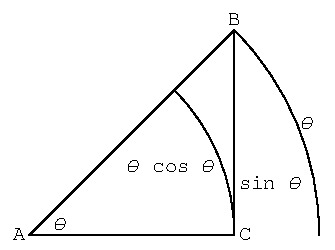
\includegraphics[width=0.4\textwidth]{calculus/differential/sintheta}
      \end{center}
      \caption{Demonstration of the inequality.}
      \label{sintheta}
    \end{figure}

    Considering the length of these three curves
    gives us the inequality:
    \[
    \theta \cos \theta \leq \sin \theta \leq \theta.
    \]
    Dividing by $\theta$,
    \[
    \cos \theta \leq \frac{\sin \theta}{\theta} \leq 1.
    \]
    Taking the limit as $\theta \to 0$ gives us
    \[
    \lim_{\theta \to 0} \frac{\sin \theta}{\theta} = 1.
    \]
    One more little tidbit we'll need to know is
    \begin{align*}
      \lim_{\theta \to 0} \left[ \frac{\cos \theta - 1}{\theta} \right]
      &= \lim_{\theta \to 0} \left[ \frac{\cos \theta - 1}{\theta}
        \frac{\cos \theta + 1}{\cos \theta + 1} \right] \\
      &= \lim_{\theta \to 0} \left[ \frac{\cos^2 \theta - 1}
        {\theta (\cos \theta + 1)} \right] \\
      &= \lim_{\theta \to 0} \left[ \frac{-\sin^2 \theta}
        {\theta (\cos \theta + 1)} \right] \\
      &= \lim_{\theta \to 0} \left[ \frac{-\sin \theta} {\theta} \right]
      \lim_{\theta \to 0} \left[ \frac{\sin \theta}
        {(\cos \theta + 1)} \right] \\
      &= (-1) \left( \frac{0}{2} \right) \\
      &= 0.
    \end{align*}
    Now we're ready to find the derivative of $\sin x$.
    \begin{align*}
      \frac{\dd}{\dd x} (\sin x)
      &= \lim_{\Delta x \to 0} \left[ \frac{\sin(x+\Delta x) - \sin x}
        {\Delta x} \right] \\
      &= \lim_{\Delta x \to 0} \left[ \frac{\cos x \sin \Delta x
          + \sin x \cos \Delta x - \sin x}{\Delta x} \right] \\
      &= \cos x \lim_{\Delta x \to 0} \left[ \frac{\sin \Delta x}{\Delta x}
      \right]
      + \sin x \lim_{\Delta x \to 0} \left[ \frac{\cos \Delta x - 1}
        {\Delta x} \right] \\
      &= \cos x
    \end{align*}
    \[
    \boxed{
      \frac{\dd}{\dd x} (\sin x) = \cos x
      }
    \]
    %%
  \item
    Let $u = g(x)$.
    Consider a nonzero increment $\Delta x$, which induces the increments
    $\Delta u$ and $\Delta f$.  By definition,
    \[
    \Delta f = f(u + \Delta u) - f(u), \qquad
    \Delta u = g(x + \Delta x) - g(x),
    \]
    and $\Delta f, \Delta u \to 0$ as $\Delta x \to 0$.
    If $\Delta u \neq 0$ then we have
    \[
    \epsilon = \frac{\Delta f}{\Delta u} - \frac{\dd f}{\dd u} \to 0 \quad \mathrm{as}
    \quad \Delta u \to 0.
    \]
    If $\Delta u = 0$ for some values of $\Delta x$ then $\Delta f$ also vanishes
    and we define $\epsilon = 0$ for theses values.  In either case,
    \[
    \Delta y = \frac{\dd f}{\dd u} \Delta u + \epsilon \Delta u.
    \]
    We divide this equation by $\Delta x$ and take the limit as $\Delta x \to 0$.
    \begin{align*}
      \frac{\dd f}{\dd x}
      &= \lim_{\Delta x \to 0} \frac{\Delta f}{\Delta x} \\
      &= \lim_{\Delta x \to 0} \left( \frac{\dd f}{\dd u}
        \frac{\Delta u}{\Delta x} + \epsilon \frac{\Delta u}{\Delta x}
      \right) \\
      &= \left( \frac{\dd f}{\dd u} \right) \left( \lim_{\Delta x \to 0}
        \frac{\Delta f}{\Delta x} \right) +
      \left( \lim_{\Delta x \to 0} \epsilon \right)
      \left( \lim_{\Delta x \to 0} \frac{\Delta u}{\Delta x} \right) \\
      &= \frac{\dd f}{\dd u} \frac{\dd u}{\dd x} +
      \left( 0 \right) \left( \frac{\dd u}{\dd x} \right) \\
      &= \frac{\dd f}{\dd u} \frac{\dd u}{\dd x}
    \end{align*}
    Thus we see that
    \[
    \boxed{
      \frac{\dd}{\dd x} (f(g(x))) = f'(g(x)) g'(x).
      }
    \]
  \end{enumerate}
  \renewcommand{\theenumi}{\arabic{enumi}}
\end{Solution}







\begin{Solution}
  \label{solution differentiable f = x|x|}
  \begin{enumerate}
  \item
    \begin{align*}
      f'(0) &= \lim_{\epsilon \to 0} \frac{\epsilon |\epsilon| - 0}{\epsilon}
      \\
      &= \lim_{\epsilon \to 0} |\epsilon|
      \\
      &= 0
    \end{align*}
    The function is differentiable at $x = 0$.
  \item
    \begin{figure}[tb]
      \begin{center}
        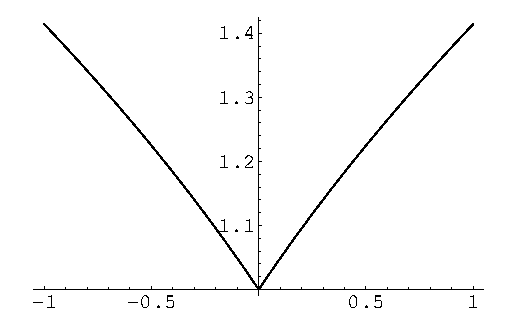
\includegraphics[width=0.4\textwidth]{calculus/differential/sqrt1x}
      \end{center}
      \caption{The function is not differentiable at the origin.}
      \label{figure sqrt1x}
    \end{figure}

    If we plot $\sqrt{1 + |x|}$, we can see that it is not differentiable 
    at $x = 0$ - it has a corner there.  
    (See Figure~\ref{figure sqrt1x}.)  The plot does not suffice for 
    demonstrating that the derivative does not exist.  However, it gives 
    us some useful insight.  We can see that the function is differentiable
    to the left and right of $x = 0$, but the slopes are different as 
    we approach the origin from the two directions.  
    Recall the definition of the derivative:
    \[
    f'(0) = \lim_{\epsilon \to 0} \frac{\sqrt{1 + |\epsilon|} - 1}{\epsilon}.
    \]
    We will show that the limit does not exist by demonstrating that 
    the left and right limits have different values.
    (The limit exists if and only if the left and right limits exist and 
    are equal.)  First consider the right limit.
    \[
    \lim_{\epsilon \to 0^+} \frac{\sqrt{1 + |\epsilon|} - 1}{\epsilon}
    = \lim_{\epsilon \to 0^+} \frac{\sqrt{1 + \epsilon} - 1}{\epsilon}
    \]
    Note that $\sqrt{1 + \epsilon} \geq 1 + \epsilon / 3$ for $\epsilon \in [0 .. 3]$.
    (See Figure~\ref{figure sqrt1x1x3}.)  This lets us get a lower bound 
    on the limit.
    \[
    \lim_{\epsilon \to 0^+} \frac{\sqrt{1 + \epsilon} - 1}{\epsilon}
    \geq \lim_{\epsilon \to 0^+} \frac{1 + \epsilon / 3 - 1}{\epsilon} = \frac{1}{3}
    \]

    \begin{figure}[tb]
      \begin{center}
        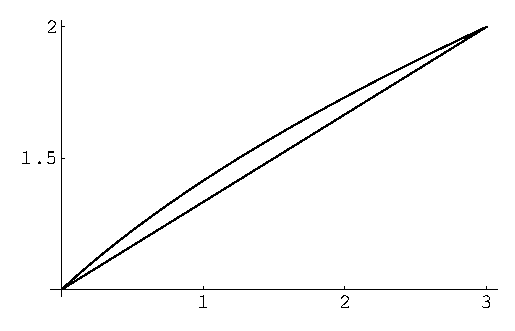
\includegraphics[width=0.4\textwidth]{calculus/differential/sqrt1x1x3}
      \end{center}
      \caption{A lower bound on the function.}
      \label{figure sqrt1x1x3}
    \end{figure}

    Now consider the left limit.
    \begin{align*}
      \lim_{\epsilon \to 0^-} \frac{\sqrt{1 + |\epsilon|} - 1}{\epsilon}
      &= \lim_{\epsilon \to 0^+} \frac{\sqrt{1 + \epsilon} - 1}{-\epsilon}
      \\
      &\leq \lim_{\epsilon \to 0^+} - \frac{1 + \epsilon / 3 - 1}{\epsilon} 
      \\
      &= -\frac{1}{3}
    \end{align*}
    Since the right limit is greater than or equal to $1/3$ and the left 
    limit is less than or equal to $- 1 / 3$, the limit does not exist.
    We conclude that $f(x) = \sqrt{1 + |x}$ is not differentiable 
    at $x = 0$.

    The problem is easier if we use L'Hospital's rule.  We can differentiate
    the numerator and denominator for $\epsilon \neq 0$.
    \begin{align*}
      f'(0) &= \lim_{\epsilon \to 0} \frac{\sqrt{1 + |\epsilon|} - 1}{\epsilon}
      \\
      &= \lim_{\epsilon \to 0} \frac{\frac{1}{2} (1 + |\epsilon|)^{-1/2} \sign(\epsilon)}{1}
      \\
      &= \lim_{\epsilon \to 0} \frac{1}{2} \sign(\epsilon)
    \end{align*}
    Since the limit does not exist,
    we conclude that the function is not differentiable at $x = 0$.
    However, since we haven't covered L'Hospital's rule yet, the 
    elementary method is more appropriate.
  \end{enumerate}
\end{Solution}



\begin{Solution}
  \label{solution d/dx x sin cos x}
  \renewcommand{\theenumi}{\alph{enumi}}
  \begin{enumerate}
    %%
  \item
    \begin{align*}
      \frac{\dd}{\dd x} [x \sin( \cos x) ]
      &= \frac{\dd}{\dd x} [x] \sin( \cos x ) + x \frac{\dd}{\dd x} [\sin(\cos x)]\\
      &= \sin( \cos x ) + x \cos(\cos x) \frac{\dd}{\dd x} [\cos x] \\
      &= \sin( \cos x ) - x \cos(\cos x) \sin x
    \end{align*}
    \[
    \boxed{
      \frac{\dd}{\dd x} [x \sin( \cos x) ] = \sin( \cos x ) - x \cos(\cos x) \sin x
      }
    \]
    %%
  \item
    \begin{align*}
      \frac{\dd}{\dd x} [f(\cos(g(x)))]
      &= f'(\cos(g(x))) \frac{\dd}{\dd x} [\cos(g(x))] \\
      &= - f'(\cos(g(x))) \sin(g(x)) \frac{\dd}{\dd x} [g(x)] \\
      &= - f'(\cos(g(x))) \sin(g(x)) g'(x)
    \end{align*}
    \[
    \boxed{
      \frac{\dd}{\dd x} [f(\cos(g(x)))] = - f'(\cos(g(x))) \sin(g(x)) g'(x)
      }
    \]
    %%
  \item
    \begin{align*}
      \frac{\dd}{\dd x} \left[ \frac{1}{f(\ln x)} \right]
      &= - \frac{ \frac{\dd}{\dd x} [ f(\ln x) ] }{ [f(\ln x) ]^2 } \\
      &= - \frac{ f'(\ln x) \frac{\dd}{\dd x} [\ln x] }{ [f(\ln x) ]^2 } \\
      &= - \frac{ f'(\ln x) }{ x [f(\ln x) ]^2 }
    \end{align*}
    \[
    \boxed{
      \frac{\dd}{\dd x} \left[ \frac{1}{f(\ln x)} \right]
      = - \frac{ f'(\ln x) }{ x [f(\ln x) ]^2 }
      }
    \]
    %%
  \item
    First we write the expression in terms exponentials and logarithms,
    \[
    x^{x^x} = x^{\exp( x \ln x)} = \exp( \exp( x \ln x ) \ln x ).
    \]
    Then we differentiate using the chain rule and the product rule.
    \begin{align*}
      \frac{\dd}{\dd x} \exp( \exp( x \ln x ) \ln x )
      &= \exp( \exp( x \ln x ) \ln x )
      \frac{\dd}{\dd x} (\exp( x \ln x ) \ln x ) \\
      &= x^{x^x} \left(
        \exp( x \ln x ) \frac{\dd}{\dd x} (x \ln x ) \ln x  +
        \exp( x \ln x ) \frac{1}{x} \right) \\
      &= x^{x^x} \left(
        x^x (\ln x + x \frac{1}{x}) \ln x  +
        x^{-1} \exp( x \ln x ) \right) \\
      &= x^{x^x} \left(
        x^x (\ln x + 1) \ln x  + x^{-1} x^x \right) \\
      &= x^{x^x + x} \left( x^{-1} + \ln x + \ln^2 x \right)
    \end{align*}
    \[
    \boxed{
      \frac{\dd}{\dd x} x^{x^x}
      = x^{x^x + x} \left( x^{-1} + \ln x + \ln^2 x \right)
      }
    \]
    %%
  \item
    We will use the fact that the sine is an odd function, i.e. 
    $\sin(-x) = - \sin x$.
    For $x \geq 0$, the expression is $x \sin x$;  for $x \leq 0$, the expression
    is $(-x) \sin(-x) = x \sin x$.  Thus we see that
    \[
    |x| \sin |x| = x \sin x.
    \]
    The first derivative of this is
    \[
    \sin x + x \cos x.
    \]
    \[
    \boxed{
      \frac{\dd}{\dd x} (|x| \sin |x| ) = \sin x + x \cos x
      }
    \]
  \end{enumerate}
  \renewcommand{\theenumi}{\arabic{enumi}}
\end{Solution}






\begin{Solution}
  \label{solution d/dx arcsin x}
  Let $y(x) = \arcsin x$.  Then $x = \sin y$.  We start with the derivative 
  of $\sin y$.
  \[
  \frac{\dd}{\dd y} \sin y = \cos y
  \]
  We substitute $x = \sin y$ and then take the multiplicative inverse to 
  get an expression for the derivative of the inverse sine.
  \begin{gather*}
    \frac{\dd x}{\dd y} = \cos y
    \\
    \frac{\dd}{\dd x} \arcsin x = \frac{1}{\cos y} 
  \end{gather*}
  Then we write the expression in terms of $x$.
  \begin{gather*}
    \frac{\dd}{\dd x} \arcsin x = \frac{1}{(1 - \sin^2 y)^{1/2}} 
    \\
    \boxed{
      \frac{\dd}{\dd x} \arcsin x = \frac{1}{(1 - x^2)^{1/2}}
    }
  \end{gather*}

  We follow the same steps to find the derivative of the inverse tangent.
  Let $y(x) = \arctan x$.  Then $x = \tan y$.  We start with the derivative 
  of the tangent.
  \begin{gather*}
    \frac{\dd}{\dd y} \tan y = \frac{1}{\cos^2 y}
    \\
    \frac{\dd x}{\dd y} = \frac{1}{\cos^2 y}
    \\
    \frac{\dd}{\dd x} \arctan x = \cos^2 y
    \\
    \frac{\dd}{\dd x} \arctan x = \cos^2 (\arctan x)
  \end{gather*}
  Now we use that $\cos(\arctan x) = (1 + x^2)^{1/2}$.  
  (The easiest way to remember these identities is to draw the 
  appropriate right triangle.  See Figure~\ref{figure cosarctanx}.)
  \begin{gather*}
    \frac{\dd}{\dd x} \arctan x = \left( \frac{1}{(1+x^2)^{1/2}} \right)^2
    \\
    \boxed{
      \frac{\dd}{\dd x} \arctan x = \frac{1}{1 + x^2}
    }
  \end{gather*}

  \begin{figure}[tb]
    \begin{center}
      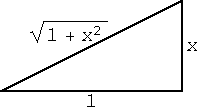
\includegraphics[width=0.2\textwidth]{calculus/differential/cosarctanx}
    \end{center}
    \caption{The triangle for determining the cosine of the inverse tangent.}
    \label{figure cosarctanx}
  \end{figure}
\end{Solution}











%%-----------------------------------------------------------------------------
%% Implicit Differentiation




\begin{Solution}
  \label{solution tangent circle}
  We differentiate the equation of the circle with respect to $x$.
  \begin{gather*}
    x^2 + y^2 = 1
    \\
    2 x + 2 y y' = 0
  \end{gather*}
  We can solve this equation for $y'(x)$.
  \[
  y'(x) = - \frac{x}{y(x)}
  \]
  To find $y'(1/2)$ we need to find $y(x)$ in terms of $x$.
  \begin{gather*}
    y(x) = \pm \sqrt{1 - x^2}
    \\
    y'(x) = \pm \frac{x}{\sqrt{1 - x^2}}
  \end{gather*}
  $y'(1/2)$ can have the two values:
  \[
  \boxed{
    y' \left( \frac{1}{2} \right) = \pm \frac{1}{\sqrt{3}}.
    }
  \]
\end{Solution}






\begin{Solution}
  \label{solution y' y'' circle}
  We differentiate the equation and solve for $y'(x)$.
  \begin{gather*}
    x^2 - x y + y^2 = 3
    \\
    2 x - y - x y' + 2 y y' = 0
    \\
    \boxed{
      y'(x) = \frac{y - 2 x}{2 y - x}
    }
  \end{gather*}
  Then we differentiate $y'(x)$ to get $y''(x)$.
  \begin{gather*}
    y''(x) = \frac{(y' - 2)(2 y - x) - (y - 2 x)(2y' - 1)}{(2 y - x)^2}
    \\
    y''(x) = 3 \frac{x y' - y }{(2 y - x)^2}
    \\
    \intertext{We substitute the solution we found for $y'$.}
    y''(x) = 3 \frac{x \frac{y - 2 x}{2 y - x} - y}{(2 y - x)^2}
    \\
    y''(x) = 3 \frac{x (y - 2 x) - y (2 y - x) }{(2 y - x)^3}
    \\
    y''(x) = - 6 \frac{x^2 - x y + y^2}{(2 y - x)^3}
    \\
    \intertext{Finally we use the original equation to simplify the numerator.}
    \boxed{
      y''(x) =  - \frac{18}{(2 y - x)^3}
    }
  \end{gather*}
\end{Solution}



%%-----------------------------------------------------------------------------
%% Maxima and Minima



\begin{Solution}
  \label{solution max min x(12-2x)2}
  \renewcommand{\theenumi}{\alph{enumi}}
  \begin{enumerate}
    %%
  \item
    First we differentiate the function.
    \[
    f(x) = x (12 - 2 x)^2
    \]
    \begin{align*}
      f'(x)
      &= (12 - 2 x)^2 + 2 x (12 - 2 x) (-2) 
      \\
      &= 4 (x - 6)^2 + 8 x (x - 6) 
      \\
      &= 12 (x - 2)(x - 6)
    \end{align*}
    By solving $f'(x) = 0$, we see that there are critical points at 
    $x = 2$ and $x = 6$.  Next we compute the second derivative to attempt
    to determine the nature of the critical points.
    \begin{gather*}
      f''(x) = 12 (x - 2) + 12 (x - 6) = 24 (x - 4)
      \\
      f''(2) = - 48, \quad f''(6) = 48
    \end{gather*}
    Since $f''(2)$ is negative, $x = 2$ is a local maximum. 
    Since $f''(6)$ is positive, $x = 6$ is a local minimum. 
    The plot of the function in Figure~\ref{figure minmax-x122x2} corroborates
    this.

    \begin{figure}[tb]
      \begin{center}
        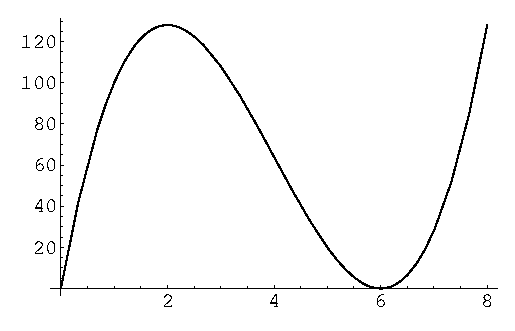
\includegraphics[width=0.4\textwidth]{calculus/differential/minmax-x122x2}
        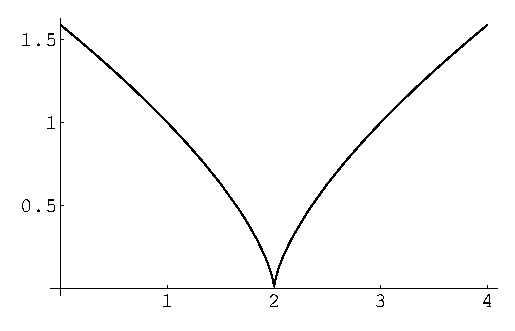
\includegraphics[width=0.4\textwidth]{calculus/differential/minmax-3x22}
      \end{center}
      \caption{The maxima and minima of the functions.}
      \label{figure minmax-x122x2}
    \end{figure}
    %%
  \item
    First we differentiate the function to try to find critical points.
    \begin{gather*}
      f(x) = \sqrt[3]{(x - 2)^2}
      \\
      f'(x) = \frac{1}{3} \left( (x - 2)^2 \right)^{-2/3} 2 (x - 2)
      \\
      f'(x) = \frac{ 2 (x - 2) }{ 3 \sqrt[3]{(x - 2)^4} }
    \end{gather*}
    The first derivative exists and is nonzero for $x \neq 2$.  At $x = 2$, the
    derivative does not exist and thus $x = 2$ is a critical point.  For 
    $x < 2$, $f'(x) < 0$ and for $x > 2$, $f'(x) > 0$.
    Thus $x = 2$ is a local minimum.
    (See the second plot in Figure~\ref{figure minmax-x122x2}.)
  \end{enumerate}
  \renewcommand{\theenumi}{\arabic{enumi}}
\end{Solution}








\begin{Solution}
  \label{solution surface area cup}
  Let $r$ be the radius and $h$ the height of the cylinder.  The volume of
  the cup is $\pi r^2 h = 64$.  Thus the radius and height are related by
  $h = \frac{64}{\pi r^2}$.  We write the surface area of the cup as a 
  function of $r$.
  \[
  f(r) = \pi r^2 + 2 \pi r h = \pi r^2 + \frac{128}{r}
  \]
  We compute the first derivative of the surface area and equate 
  it to zero to find the critical points.
  \begin{gather*}
    f'(r) = 2 \pi r - \frac{128}{r^2} = 0
    \\
    2 \pi r^3 - 128 = 0
    \\
    \intertext{This cubic equation has a single real root.}
    r = \frac{4}{\sqrt[3]{\pi}}
  \end{gather*}
  The second derivative of the surface area is
  $f''(r) = 2 \pi + \frac{256}{r^3}$.  Since
  $f''(\frac{4}{\sqrt[3]{\pi}}) = 6\pi$, $r=\frac{4}{\sqrt[3]{\pi}}$ is a
  local minimum of $f(r)$.  Since this is the only critical point for
  real-valued $r$, it must be a global minimum.
  The cup has a radius of $\frac{4}{\sqrt[3]{\pi}}$ cm and a height of
  $\frac{4}{\sqrt[3]{\pi}}$ cm.
\end{Solution}



%%-----------------------------------------------------------------------------
%% Mean Value Theorems


\begin{Solution}
  \label{solution generalized theorem of the mean}
  We will use Rolle's theorem to prove the generalized theorem of the 
  mean.  First we need to define a function $h(x)$ that is differentiable
  and vanishes at $x = a$ and $x = b$.
  \[
  h(x) = f(x) - f(a) - \frac{f(b) - f(a)}{g(b) - g(a)} (g(x) - g(a)).
  \]
  Since $h(x)$ satisfies the conditions of Rolle's theorem, there exists a 
  point $\xi \in (a,b)$ where $h'(\xi) = 0$.
  \begin{gather*}
    h'(\xi) = f'(\xi) - \frac{f(b) - f(a)}{g(b) - g(a)} g'(\xi) = 0
    \\
    \frac{f'(\xi)}{g'(\xi)} = \frac{f(b) - f(a)}{g(b) - g(a)}
  \end{gather*}
\end{Solution}



\begin{Solution}
  \label{solution polynomial approximation sin x}
  The first few terms in the Taylor series of $\sin(x)$ about $x = 0$ are
  \[
  \sin(x) = x - \frac{x^3}{6} + \frac{x^5}{120} - \frac{x^7}{5040}
  + \frac{x^9}{362880} + \cdots.
  \]
  The seventh derivative of $\sin x$ is $-\cos x$.  Thus 
  \[
  \sin(x) = x - \frac{x^3}{6} + \frac{x^5}{120} - \frac{\cos x_0}{5040} x^7,
  \]
  where $x_0$ is in the interval $[0 .. x]$.  
  Since we are considering $x \in [-1,1]$ and
  $-1 \leq \cos(x_0) \leq 1$, the approximation
  \[
  \boxed{
    \sin x \approx x - \frac{x^3}{6} + \frac{x^5}{120}
    }
  \]
  has a maximum error of $\frac{1}{5040} \approx 0.000198$.
  We use this polynomial to approximate $\sin(1)$
  and verify that it has the required accuracy.
  \begin{gather*}
    \boxed{
      1 - \frac{1^3}{6} + \frac{1^5}{120} \approx 0.841667
    }
    \\
    \sin(1) \approx 0.841471
  \end{gather*}
  See Figure~\ref{figure sin-app} for plots of various polynomial 
  approximations of $\sin x$.
  \begin{figure}[tb]
    \begin{center}
      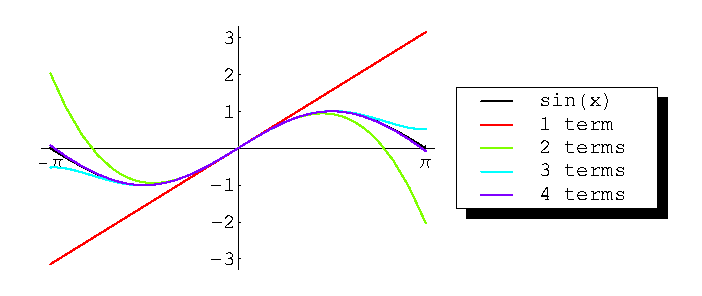
\includegraphics[width=0.9\textwidth]{calculus/differential/sin-app}
    \end{center}
    \caption{Polynomial approximations of the sine.}
    \label{figure sin-app}
  \end{figure}
\end{Solution}




\begin{Solution}
  \label{solution second difference centered}
  Expanding the terms in the approximation in Taylor series,
  \begin{align*}
    f(x+\Delta x) &= f(x) + \Delta x f'(x) + \frac{\Delta x^2}{2} f''(x)
    +\frac{\Delta x^3}{6} f'''(x) + \frac{\Delta x^4}{24} f''''(x_1), \\
    f(x-\Delta x) &= f(x) - \Delta x f'(x) + \frac{\Delta x^2}{2} f''(x)
    -\frac{\Delta x^3}{6} f'''(x) + \frac{\Delta x^4}{24} f''''(x_2),
  \end{align*}
  where $x \leq x_1 \leq x + \Delta x$ and $x - \Delta x \leq x_2 \leq x$.
  Substituting the expansions into the formula,
  \[
  \frac{f(x+\Delta x) - 2 f(x) + f(x-\Delta x)}{\Delta x^2}
  = f''(x) + \frac{\Delta x^2}{24} [f''''(x_1) + f''''(x_2)].
  \]
  Thus the error in the approximation is
  \[
  \boxed{
    \frac{\Delta x^2}{24} [f''''(x_1) + f''''(x_2)].
    }
  \]
\end{Solution}




\begin{Solution}
  \label{solution first derivative higher}
  %% CONTINUE
\end{Solution}



%%-----------------------------------------------------------------------------
%% L'Hospital's Rule





\begin{Solution}
  \label{solution lim (x - sin x)/x3}
  \renewcommand{\theenumi}{\alph{enumi}}
  \begin{enumerate}
    %%
  \item
    \begin{align*}
      \lim_{x \to 0} \left[ \frac{x-\sin x}{x^3} \right]
      &= \lim_{x \to 0} \left[ \frac{1-\cos x}{3 x^2} \right] \\
      &= \lim_{x \to 0} \left[ \frac{\sin x}{6 x} \right] \\
      &= \lim_{x \to 0} \left[ \frac{\cos x}{6} \right] \\
      &= \frac{1}{6}
    \end{align*}
    \[
    \boxed{
      \lim_{x \to 0} \left[ \frac{x-\sin x}{x^3} \right] = \frac{1}{6}
      }
    \]
    %%
  \item
    \begin{align*}
      \lim_{x \to 0} \left( \csc x - \frac{1}{x} \right)
      &= \lim_{x \to 0} \left( \frac{1}{\sin x} - \frac{1}{x} \right) \\
      &= \lim_{x \to 0} \left( \frac{x - \sin x}{x \sin x} \right) \\
      &= \lim_{x \to 0} \left( \frac{1 - \cos x}{x \cos x + \sin x} \right)\\
      &= \lim_{x \to 0} \left( \frac{\sin x}{- x \sin x + \cos x + \cos x}
      \right) \\
      &= \frac{0}{2} \\
      &= 0
    \end{align*}
    \[
    \boxed{
      \lim_{x \to 0} \left( \csc x - \frac{1}{x} \right) = 0
      }
    \]
    %%
  \item
    \begin{align*}
      \ln\left( \lim_{x \to +\infty} \left[ \left(1 + \frac{1}{x} \right)^x
        \right] \right)
      &= \lim_{x \to +\infty} \left[ \ln\left( \left(1 + \frac{1}{x}
          \right)^x \right) \right] \\
      &= \lim_{x \to +\infty} \left[ x \ln\left(1+\frac{1}{x}\right)
      \right] \\
      &= \lim_{x \to +\infty} \left[ \frac{\ln\left(1+\frac{1}{x}\right)}
        {1/x} \right] \\
      &= \lim_{x \to +\infty} \left[ \frac{\left(1+\frac{1}{x}\right)^{-1}
          \left(-\frac{1}{x^2}\right)}
        {-1/x^2} \right] \\
      &= \lim_{x \to +\infty} \left[ \left(1+\frac{1}{x}\right)^{-1}
      \right] \\
      &= 1
    \end{align*}
    Thus we have
    \[
    \boxed{
      \lim_{x \to +\infty} \left[ \left(1 + \frac{1}{x} \right)^x \right] = e.
      }
    \]
    %%
  \item
    It takes four successive applications of L'Hospital's rule to evaluate
    the limit.
    \begin{align*}
      \lim_{x \to 0} \left( \csc^2 x - \frac{1}{x^2} \right)
      &= \lim_{x \to 0} \frac{x^2 - \sin^2 x}{ x^2 \sin^2 x } \\
      &= \lim_{x \to 0} \frac{ 2 x - 2 \cos x \sin x }
      { 2 x^2 \cos x \sin x + 2 x \sin^2 x } \\
      &= \lim_{x \to 0} \frac{2 - 2 \cos^2 x + 2 \sin^2 x }
      { 2 x^2 \cos^2 x + 8 x \cos x \sin x + 2 \sin^2 x
        - 2 x^2 \sin^2 x } \\
      &= \lim_{x \to 0} \frac{ 8 \cos x \sin x }
      { 12 x \cos^2 x + 12 \cos x \sin x - 8 x^2 \cos x \sin x
        - 12 x \sin^2 x } \\
      &= \lim_{x \to 0} \frac{ 8 \cos^2 x - 8 \sin^2 x }
      { 24 \cos^2 x - 8 x^2 \cos^2 x - 64 x \cos x \sin x
        - 24 \sin^2 x + 8 x^2 \sin^2 x } \\
      &= \frac{1}{3}
    \end{align*}

    It is easier to use a Taylor series expansion.
    \begin{align*}
      \lim_{x \to 0} \left( \csc^2 x - \frac{1}{x^2} \right)
      &= \lim_{x \to 0} \frac{x^2 - \sin^2 x}{ x^2 \sin^2 x } \\
      &= \lim_{x \to 0} \frac{x^2 - (x - x^3/6 + O(x^5))^2}
      { x^2 (x + O(x^3))^2 } \\
      &= \lim_{x \to 0} \frac{x^2 - (x^2 - x^4/3 + O(x^6))}
      { x^4 + O(x^6) } \\
      &= \lim_{x \to 0} \left( \frac{1}{3} + O(x^2) \right) \\
      &= \frac{1}{3}
    \end{align*}
  \end{enumerate}
  \renewcommand{\theenumi}{\arabic{enumi}}
\end{Solution}






\begin{Solution}
  \label{solution lim x a/x}
  To evaluate the first limit, we use the identity $a^b = \e^{b \ln a}$
  and then apply L'Hospital's rule.
  \begin{align*}
    \lim_{x \to \infty} x^{a/x}
    &= \lim_{x \to \infty} \e^{\frac{a \ln x}{x} } \\
    &= \exp \left( \lim_{x \to \infty} \frac{a \ln x}{x} \right) \\
    &= \exp \left( \lim_{x \to \infty} \frac{a / x}{1} \right) \\
    &= \e^0
  \end{align*}
  \[
  \boxed{
    \lim_{x \to \infty} x^{a/x} = 1
    }
  \]

  We use the same method to evaluate the second limit.
  \begin{align*}
    \lim_{x \to \infty} \left( 1 + \frac{a}{x} \right)^{b x}
    &= \lim_{x \to \infty} \exp \left( b x
      \ln \left( 1 + \frac{a}{x} \right) \right) \\
    &= \exp \left( \lim_{x \to \infty} b x
      \ln \left( 1 + \frac{a}{x} \right) \right) \\
    &= \exp \left( \lim_{x \to \infty} b
      \frac{\ln( 1 + a/x )}{1/x} \right) \\
    &= \exp \left( \lim_{x \to \infty} b
      \frac{\frac{-a/x^2}{1+a/x}}{-1/x^2} \right) \\
    &= \exp \left( \lim_{x \to \infty} b
      \frac{a}{1+a/x} \right)
  \end{align*}
  \[
  \boxed{
    \lim_{x \to \infty} \left( 1 + \frac{a}{x} \right)^{b x} = \e^{a b}
    }
  \]
\end{Solution}








\raggedbottom
%%=============================================================================
\pagebreak
\flushbottom
\section{Quiz}

\begin{QuizProblem}
  \label{quiz problem define continuity}
  Define \textit{continuity}.

  \quizsolution{define continuity}
\end{QuizProblem}


\begin{QuizProblem}
  \label{quiz problem necessary sufficient continuity differentiability}
  Fill in the blank with \textit{necessary}, \textit{sufficient} or
  \textit{necessary and sufficient}.

  Continuity is a $\underline{\phantom{necessary and sufficient}}$ condition 
  for differentiability.

  Differentiability is a $\underline{\phantom{necessary and sufficient}}$ 
  condition for continuity.

  Existence of $\lim_{\Delta x \to 0} \frac{f(x+\Delta x) - f(x)}{\Delta x}$ is a 
  $\underline{\phantom{necessary and sufficient}}$ condition for
  differentiability.

  \quizsolution{necessary sufficient continuity differentiability}
\end{QuizProblem}


\begin{QuizProblem}
  \label{quiz problem ddx f(g(x)h(x))}
  Evaluate $\frac{\dd}{\dd x} f(g(x) h(x))$.

  \quizsolution{ddx f(g(x)h(x))}
\end{QuizProblem}


\begin{QuizProblem}
  \label{quiz problem ddx f(x)g(x)}
  Evaluate $\frac{\dd}{\dd x} f(x)^{g(x)}$.

  \quizsolution{ddx f(x)g(x)}
\end{QuizProblem}


\begin{QuizProblem}
  \label{quiz problem theorem of the mean}
  State the Theorem of the Mean.  Interpret the theorem physically.

  \quizsolution{theorem of the mean}
\end{QuizProblem}


\begin{QuizProblem}
  \label{quiz problem taylor's theorem of the mean}
  State Taylor's Theorem of the Mean.

  \quizsolution{taylor's theorem of the mean}
\end{QuizProblem}


\begin{QuizProblem}
  \label{quiz problem lim sin sin}
  Evaluate $\lim_{x \to 0} (\sin x)^{\sin x}$.

  \quizsolution{lim sin sin}
\end{QuizProblem}









\raggedbottom
%%=============================================================================
\pagebreak
\flushbottom
\section{Quiz Solutions}


\begin{QuizSolution}
  \label{quiz solution define continuity}
  A function $y(x)$ is said to be \textit{continuous at} $x = \xi$ if
  $\lim_{x \to \xi} y(x) = y(\xi)$. 
\end{QuizSolution}


\begin{QuizSolution}
  \label{quiz solution necessary sufficient continuity differentiability}
  Continuity is a necessary condition for differentiability.

  Differentiability is a sufficient condition for continuity.

  Existence of $\lim_{\Delta x \to 0} \frac{f(x+\Delta x) - f(x)}{\Delta x}$ is a 
  necessary and sufficient condition for differentiability.
\end{QuizSolution}


\begin{QuizSolution}
  \label{quiz solution ddx f(g(x)h(x))}
  \[
  \frac{\dd}{\dd x} f(g(x) h(x)) 
  = f'(g(x) h(x)) \frac{\dd}{\dd x} (g(x) h(x))
  = f'(g(x) h(x)) (g'(x) h(x) + g(x) h'(x))
  \]
\end{QuizSolution}


\begin{QuizSolution}
  \label{quiz solution ddx f(x)g(x)}
  \begin{align*}
    \frac{\dd}{\dd x} f(x)^{g(x)} 
    &= \frac{\dd}{\dd x} e^{g(x) \ln f(x)} 
    \\
    &= \e^{g(x) \ln f(x)} \frac{\dd}{\dd x} (g(x) \ln f(x)) 
    \\
    &= f(x)^{g(x)} \left( g'(x) \ln f(x) + g(x) \frac{f'(x)}{f(x)} \right)
  \end{align*}
\end{QuizSolution}


\begin{QuizSolution}
  \label{quiz solution theorem of the mean}
  If $f(x)$ is continuous in $[a..b]$ and differentiable in $(a..b)$ 
  then there exists a point $x = \xi$ such that
  \[
  f'(\xi) = \frac{f(b) - f(a)}{b - a}.
  \]
  That is, there is a point where the instantaneous velocity is equal to
  the average velocity on the interval. 
\end{QuizSolution}


\begin{QuizSolution}
  \label{quiz solution taylor's theorem of the mean}
  If $f(x)$ is $n+1$ times continuously differentiable in $(a..b)$ 
  then there exists a point $x = \xi \in (a..b)$ such that
  \[
  f(b) = f(a) + (b-a) f'(a) + \frac{(b-a)^2}{2!} f''(a) + \cdots +
  \frac{(b-a)^n}{n!} f^{(n)}(a)
  + \frac{(b-a)^{n+1}}{(n+1)!} f^{(n+1)}(\xi).
  \]
\end{QuizSolution}


\begin{QuizSolution}
  \label{quiz solution lim sin sin}
  Consider $\lim_{x \to 0} (\sin x)^{\sin x}$.  This is an indeterminate of 
  the form $0^0$.  The limit of the logarithm of the expression is
  $\lim_{x \to 0} \sin x \ln( \sin x )$.
  This is an indeterminate of the form $0 \cdot \infty$.  We can rearrange
  the expression to obtain an indeterminate of the form $\frac{\infty}{\infty}$
  and then apply L'Hospital's rule.
  \[
  \lim_{x \to 0} \frac{\ln( \sin x )}{1/\sin x} 
  = \lim_{x \to 0} \frac{ \cos x / \sin x}{ -\cos x / \sin^2 x }
  = \lim_{x \to 0} (- \sin x)
  = 0
  \]
  The original limit is
  \[
  \lim_{x \to 0} (\sin x)^{\sin x} = \e^0 = 1.
  \]
\end{QuizSolution}



\raggedbottom



